% latbibdo  template

\newcommand\apjcls{1}
\newcommand\aastexcls{2}
\newcommand\othercls{3}

% Select ony one pair of \papercls and class file:

% AASTEX61 cls:
\newcommand\papercls{\aastexcls}
\documentclass[tighten, times, twocolumn]{aastex62}  % ApJ look-alike
%\documentclass[tighten, times, trackchanges, twocolumn]{aastex62}
%\documentclass[tighten, times, manuscript]{aastex62} % Onecolumn, doublespaced

% Emulate ApJ cls:
%\newcommand\papercls{\apjcls}
%\documentclass[iop]{emulateapj}

% Other cls:
%\newcommand\papercls{\othercls}
%\documentclass[letterpaper,12pt]{article}


%% :::::::::::::::::::::::::::::::::::::::::::::::::::::::::::::::::::
% These are latex packages that enable various capability.

\if\papercls \apjcls
\usepackage{apjfonts}
\else\if\papercls \othercls
\usepackage{epsfig}
\usepackage{margin}
% times font (for \othercls):
\usepackage{times}
\fi\fi
\usepackage{ifthen}
\usepackage{natbib}
\usepackage{amssymb, amsmath}
\usepackage{appendix}
\usepackage{etoolbox}
\usepackage[T1]{fontenc}
\usepackage{paralist}

% This one defines a few more journals (DPS and AAS abstracts) for bibtex:
\if\papercls \apjcls
\newcommand\aas{\ref@jnl{AAS Meeting Abstracts}}% *** added by jh
          % American Astronomical Society Meeting Abstracts
\newcommand\dps{\ref@jnl{AAS/DPS Meeting Abstracts}}% *** added by jh
          % American Astronomical Society/Division for Planetary Sciences Meeting Abstracts
\newcommand\maps{\ref@jnl{MAPS}}% *** added by jh
          % Meteoritics and Planetary Science
\else\if\papercls \othercls
\usepackage{astjnlabbrev-jh}
\fi\fi

% Bibliographystyle chooses a bibtex .bst file, which defines the
% format of the references.  It's important to pick one that works for
% the journal you are writing for and that has hyperlinks for the
% actual paper online.
\bibliographystyle{apj_hyperref}
%\bibliographystyle{aasjournal}

% Enable this for packed reference list:
%\setlength\bibsep{0.0pt}

% Enable this to remove section numbers:
%\setcounter{secnumdepth}{0}

%% % Enable this for bullet-point separated references:
%% \usepackage{paralist}
%% \renewenvironment{thebibliography}[1]{\let\par\relax%
%%   \section*{\refname}\inparaitem}{\endinparaitem}
%% \let\oldbibitem\bibitem
%% \renewcommand{\bibitem}{\item[\textbullet]\oldbibitem}


% Setup hyperreferences style:
\if\papercls \aastexcls
\hypersetup{citecolor=blue, % color for \cite{...} links
            linkcolor=blue, % color for \ref{...} links
            menucolor=blue, % color for Acrobat menu buttons
            urlcolor=blue}  % color for \url{...} links
\else
\usepackage[%pdftex,      % hyper-references for pdflatex
bookmarks=true,           %%% generate bookmarks ...
bookmarksnumbered=true,   %%% ... with numbers
colorlinks=true,          % links are colored
citecolor=blue,           % color for \cite{...} links
linkcolor=blue,           % color for \ref{...} links
menucolor=blue,           % color for Acrobat menu buttons
urlcolor=blue,            % color for \url{...} links
linkbordercolor={0 0 1},  %%% blue frames around links
pdfborder={0 0 1},
frenchlinks=true]{hyperref}
\fi

% These macross generate the hyperlinks in the References section:
\if\papercls \othercls
\newcommand{\eprint}[1]{\href{http://arxiv.org/abs/#1}{#1}}
\else
\renewcommand{\eprint}[1]{\href{http://arxiv.org/abs/#1}{#1}}
\fi
\newcommand{\ISBN}[1]{\href{http://cosmologist.info/ISBN/#1}{ISBN: #1}}
\providecommand{\adsurl}[1]{\href{#1}{ADS}}

% hyper ref only the year in citations:
\makeatletter
% Patch case where name and year are separated by aysep
\patchcmd{\NAT@citex}
  {\@citea\NAT@hyper@{%
     \NAT@nmfmt{\NAT@nm}%
     \hyper@natlinkbreak{\NAT@aysep\NAT@spacechar}{\@citeb\@extra@b@citeb}%
     \NAT@date}}
  {\@citea\NAT@nmfmt{\NAT@nm}%
   \NAT@aysep\NAT@spacechar\NAT@hyper@{\NAT@date}}{}{}

% Patch case where name and year are separated by opening bracket
\patchcmd{\NAT@citex}
  {\@citea\NAT@hyper@{%
     \NAT@nmfmt{\NAT@nm}%
     \hyper@natlinkbreak{\NAT@spacechar\NAT@@open\if*#1*\else#1\NAT@spacechar\fi}%
       {\@citeb\@extra@b@citeb}%
     \NAT@date}}
  {\@citea\NAT@nmfmt{\NAT@nm}%
   \NAT@spacechar\NAT@@open\if*#1*\else#1\NAT@spacechar\fi\NAT@hyper@{\NAT@date}}
  {}{}
\makeatother

% Define lowcase: a MakeLowercase that doesn't break on subtitles:
\makeatletter
\DeclareRobustCommand{\lowcase}[1]{\@lowcase#1\@nil}
\def\@lowcase#1\@nil{\if\relax#1\relax\else\MakeLowercase{#1}\fi}
\pdfstringdefDisableCommands{\let\lowcase\@firstofone}
\makeatother

% unslanted mu, for ``micro'' abbrev.
\DeclareSymbolFont{UPM}{U}{eur}{m}{n}
\DeclareMathSymbol{\umu}{0}{UPM}{"16}
\let\oldumu=\umu
\renewcommand\umu{\ifmmode\oldumu\else\math{\oldumu}\fi}
\newcommand\micro{\umu}
\if\papercls \othercls
\newcommand\micron{\micro m}
\else
\renewcommand\micron{\micro m}
\fi
\newcommand\microns{\micron}
\newcommand\microbar{\micro bar}

% These define commands outside of math mode:
% \sim
\let\oldsim=\sim
\renewcommand\sim{\ifmmode\oldsim\else\math{\oldsim}\fi}
% \pm
\let\oldpm=\pm
\renewcommand\pm{\ifmmode\oldpm\else\math{\oldpm}\fi}
% \times
\newcommand\by{\ifmmode\times\else\math{\times}\fi}
% Ten-to-the-X and times-ten-to-the-X:
\newcommand\ttt[1]{10\sp{#1}}
\newcommand\tttt[1]{\by\ttt{#1}}

% A tablebox lets you define some lines in a block, using \\ to end
% them.  The block moves as a unit.  Good for addresses, quick lists, etc.
\newcommand\tablebox[1]{\begin{tabular}[t]{@{}l@{}}#1\end{tabular}}
% These commands are blank space exactly the width of various
% numerical components, for spacing out tables.
\newbox{\wdbox}
\renewcommand\c{\setbox\wdbox=\hbox{,}\hspace{\wd\wdbox}}
\renewcommand\i{\setbox\wdbox=\hbox{i}\hspace{\wd\wdbox}}
\newcommand\n{\hspace{0.5em}}

% \marnote puts a note in the margin:
\newcommand\marnote[1]{\marginpar{\raggedright\tiny\ttfamily\baselineskip=9pt #1}}
% \herenote makes a bold note and screams at you when you compile the
% document.  Good for reminding yourself to do something before the
% document is done.
\newcommand\herenote[1]{{\bfseries #1}\typeout{======================> note on page \arabic{page} <====================}}
% These are common herenotes:
\newcommand\fillin{\herenote{fill in}}
\newcommand\fillref{\herenote{ref}}
\newcommand\findme[1]{\herenote{FINDME #1}}

% \now is the current time.  Convenient for saying when the draft was
% last modified.
\newcount\timect
\newcount\hourct
\newcount\minct
\newcommand\now{\timect=\time \divide\timect by 60
         \hourct=\timect \multiply\hourct by 60
         \minct=\time \advance\minct by -\hourct
         \number\timect:\ifnum \minct < 10 0\fi\number\minct}

% This is pretty much like \citealp
\newcommand\citeauthyear[1]{\citeauthor{#1} \citeyear{#1}}

% These are short for multicolumn, to shorten the length of table lines.
\newcommand\mc{\multicolumn}
\newcommand\mctc{\multicolumn{2}{c}}

% Joetex character unreservations.
% This file frees most of TeX's reserved characters, and provides
% several alternatives for their functions.

% Tue Mar 29 22:23:03 EST 1994
% modified 12 Oct 2000 for AASTeX header

% utility
\catcode`@=11

% Define comment command:
\newcommand\comment[1]{}

% Undefine '%' as special character:
\newcommand\commenton{\catcode`\%=14}
\newcommand\commentoff{\catcode`\%=12}

% Undefine '$' as special character:
\renewcommand\math[1]{$#1$}
\newcommand\mathshifton{\catcode`\$=3}
\newcommand\mathshiftoff{\catcode`\$=12}

% Undefine '&' as special character:
\let\atab=&
\newcommand\atabon{\catcode`\&=4}
\newcommand\ataboff{\catcode`\&=12}

% Define \sp and \sb for superscripts and subscripts:
\let\oldmsp=\sp
\let\oldmsb=\sb
\def\sp#1{\ifmmode
           \oldmsp{#1}%
         \else\strut\raise.85ex\hbox{\scriptsize #1}\fi}
\def\sb#1{\ifmmode
           \oldmsb{#1}%
         \else\strut\raise-.54ex\hbox{\scriptsize #1}\fi}
\newbox\@sp
\newbox\@sb
\def\sbp#1#2{\ifmmode%
           \oldmsb{#1}\oldmsp{#2}%
         \else
           \setbox\@sb=\hbox{\sb{#1}}%
           \setbox\@sp=\hbox{\sp{#2}}%
           \rlap{\copy\@sb}\copy\@sp
           \ifdim \wd\@sb >\wd\@sp
             \hskip -\wd\@sp \hskip \wd\@sb
           \fi
        \fi}
\def\msp#1{\ifmmode
           \oldmsp{#1}
         \else \math{\oldmsp{#1}}\fi}
\def\msb#1{\ifmmode
           \oldmsb{#1}
         \else \math{\oldmsb{#1}}\fi}

% Undefine '^' as special character:
\def\supon{\catcode`\^=7}
\def\supoff{\catcode`\^=12}

% Undefine '_' as special character:
\def\subon{\catcode`\_=8}
\def\suboff{\catcode`\_=12}

\def\supsubon{\supon \subon}
\def\supsuboff{\supoff \suboff}

% Undefine '~' as special character:
\newcommand\actcharon{\catcode`\~=13}
\newcommand\actcharoff{\catcode`\~=12}

% Undefine '#' as special character:
\newcommand\paramon{\catcode`\#=6}
\newcommand\paramoff{\catcode`\#=12}

\comment{And now to turn us totally on and off...}

\newcommand\reservedcharson{ \commenton  \mathshifton  \atabon  \supsubon 
                             \actcharon  \paramon}

\newcommand\reservedcharsoff{\commentoff \mathshiftoff \ataboff \supsuboff 
                             \actcharoff \paramoff}

\newcommand\nojoe[1]{\reservedcharson #1 \reservedcharsoff}
\catcode`@=12
\reservedcharson


\if\papercls \apjcls
\newcommand\widedeltab{deluxetable}
\else
\newcommand\widedeltab{deluxetable*}
\fi


%% :::::::::::::::::::::::::::::::::::::::::::::::::::::::::::::::::::
%% Convenience macross:
\newcommand\tnm[1]{\tablenotemark{#1}}
%% Spitzer:
\newcommand\SST{{\em Spitzer Space Telescope}}
\newcommand\Spitzer{{\em Spitzer}}
%% chi-squared:
\newcommand\chisq{\ifmmode{\chi\sp{2}}\else\math{\chi\sp{2}}\fi}
\newcommand\redchisq{\ifmmode{ \chi\sp{2}\sb{\rm red}}
                    \else\math{\chi\sp{2}\sb{\rm red}}\fi}
%% Equilibrium temperature:
\newcommand\Teq{\ifmmode{T\sb{\rm eq}}\else$T$\sb{eq}\fi}
%% Jupiter mass, radius:
\newcommand\mjup{\ifmmode{M\sb{\rm Jup}}\else$M$\sb{Jup}\fi}
\newcommand\rjup{\ifmmode{R\sb{\rm Jup}}\else$R$\sb{Jup}\fi}
%% Solar mass, radius:
\newcommand\msun{\ifmmode{M\sb{\odot}}\else$M\sb{\odot}$\fi}
\newcommand\rsun{\ifmmode{R\sb{\odot}}\else$R\sb{\odot}$\fi}
%% Earth mass, radius:
\newcommand\mearth{\ifmmode{M\sb{\oplus}}\else$M\sb{\oplus}$\fi}
\newcommand\rearth{\ifmmode{R\sb{\oplus}}\else$R\sb{\oplus}$\fi}
%% Molecules:
\newcommand\molhyd{H$\sb{2}$}
\newcommand\methane{CH$\sb{4}$}
\newcommand\water{H$\sb{2}$O}
\newcommand\carbdiox{CO$\sb{2}$}
\newcommand\carbmono{CO}
%% Units:
\newcommand\ms{m\;s$\sp{-1}$}
\newcommand\cms{cm\;s$\sp{-1}$}

\newcommand\degree{\degr}
\newcommand\degrees{\degree}
\newcommand\vs{\emph{vs.}}


\usepackage{subfiles}
\usepackage{subfig}
% Headers for odd and even pages, respectively:
\shorttitle{ApJ Template}
% If more than two authors, use {\em et al.}
\shortauthors{Shiwu {\em et al.}}


\begin{document}

\title{Extreme outflow of Enormous Ly$\alpha$ Nebula in MAMMOTH-1}


%% AUTHOR/INSTITUTIONS FOR AASTEX6.1:
\author{Shiwu Zhang}
\affiliation{Department of Astronomy, Tsinghua University,
              Shuangqing Road No.30, Haidian Beijing China}

\author{Zheng Cai}
\affiliation{Department of Astronomy, Tsinghua University,
              Shuangqing Road No.30, Haidian Beijing China}
%% AUTHOR/INSTITUTIONS FOR EMULATE APJ:
% \author{Patricio~E.~Cubillos\altaffilmark{1,2},
% Joseph~Harrington\altaffilmark{1},
% and
% Third~Author\altaffilmark{1}
% }
% \affil{\sp{1} Planetary Sciences Group, Department of
%               Physics, University of Central Florida, Orlando, FL 32816-2385\\
%        \sp{2} Space Research Institute, Austrian Academy of Sciences,
%               Schmiedlstrasse 6, A-8042, Graz, Austria}

\email{zsw18@mails.tsinghua.edu.cn}

% %% Extra info for aastex:
% \received{Yesterday}
% \revised{Today}
% \accepted{Tonight}
% \published{Tomorrow}
% \submitjournal{AASJournal}

\begin{abstract}
  
\end{abstract}

% http://journals.aas.org/authors/keywords2013.html
\keywords{}


\section{Introduction}
\label{introduction}

Over the past few decades it has been realized that the black hole (BH) at the centre of a galaxy bulge is more than just decorations but play a key role in galaxy evolution \citep{fabian4114observational}. 
This process is known as Active Galactic Nucleus (AGN) feedback which take place by accreting matter onto the massive BH and have a profound effect on galaxy evolution even the large-scale structure comparing with the large ratio of the size of BH to host galaxy.
%The process by which this occurs is known as AGN(Active Galactic Nucleus) feedback and it takes place through an interaction between the energy and radiation generated by accretion onto the massive BH and the gas in the host galaxy. In contrast to the large ratio of the size of BH to host galaxy, AGN have a potent effect on galaxy formation and evolution even the large-scale structure. 
For example, the energy released to build a BH with mass $\rm M_{BH}=10^{8} \mathbf{M}_{\odot}$ would correspond to $\rm E_{BH} \approx 0.1M_{BH}c^{2}$. This total accretion energy is two-to-three order of magnitude higher than the binding energy of the galaxy bulge the BH reside in, and is comparable to, even higher than, the thermal energy of the gas in the dark matter halo \citep{harrison2016observational}. As a consequence, feedback induced by massive BH has the ability to change the evolution path of galaxies. Observations are required to constrain the details of when, where and how these processes actually occur.
%So the study on AGN feedback is extremely important for galaxy even cosmology.

%Theoretical models of galaxy formation and evolution have found it necessary to implement AGN feedback processes in order to produce the observational evidence. 
There are two sorts of AGN feedback mechanisms. The first one is the radio mode feedback also known as maintenance mode or kinetic mode, it is believed that this mode is the most efficient mechanism in low redshift clusters, at late times and during periods of low BH accretion rates. The objects that are responsible for this type of feedback are likely to be low-excitation radio AGN which has low accretion rate and are always companied by radio lobes \citep{churazov2005supermassive,bower2006breaking,mccarthy2011gas}. This sort of feedback is mainly used to explain the cut-off of the galaxy luminosity function in cluster environment \citep{bower2006breaking,croton2006many,somerville2008semi}. In addition, a more powerful form of interaction between AGN and its environment happens during periods of rapid accretion known as quasar mode or radiative mode. Objects which is responsible for this type of feedback are the radiatively-efficient AGN possessing large accretion rate. Theoretical models for this form of feedback typically require $\rm \approx 0.005-0.15$ of the accretion energy to couple to the cold gas within the host galaxy and to expel this gas through outflows which ultimately results in the shut-down of future BH growth or star formation \citep{benson2003shapes,hopkins2006normalization,debuhr2012galaxy}. Besides, analytical models have used the idea of galaxy-scale outflows initially launched by AGN, to explain $\rm M_{BH}-M_{bulge}$ relationship \citep{fabian1999obscured,granato2004physical,king2011large,faucher2012physics}. This form of feedback is thought to be effective at producing high mass outflow rates and quenching star formation. In addition to the potential affects of AGN feedback described above, AGN-driven outflows are required to blow the gas in their host galaxy out to explain the chemical enrichment of intercluster medium (ICM) and circumgalactic medium(CGM) \citep{borgani2008chemical,wiersma2009chemical,fabjan2010simulating,ciotti2010feedback}. In contrast, it has been prompted that, these outflows could induce positive feedback which trigger star formation by inducing pressure in cold gas reservoirs \citep{nayakshin2012quasar,ishibashi2012active,silk2013unleashing}. However, there are still many fundamental questions to be solved, it is not well established how the accretion energy couples to the gas to drive outflows and the impact of outflow on a much larger physical scale. 

%It is believed that AGN activity is required to drive the highest velocity outflows and are particularly important for the evolution of most massive galaxies(\citep{benson2003shapes};\citep{mccarthy2011gas};\citep{harrison2018agn}). 
%AGN-driven outflows are initially launched from the accretion disk or dusty torus surrounding the BH. 


Spectroscopy is used as a direct way to search for outflows. Such observations have identified outflows in ionized, atomic and molecular gas \citep{nesvadba2008evidence}. A method that is widely used to search for outflowing ionized gas is the high-velocity OIII$\rm \lambda5007$ emission line. This is a good tracer of kinematics in the narrow-line region (NLR) of AGN and people have used it to study kinematics in hundreds to ten of thousands of AGN \citep{wang2011evolution,mullaney2013narrow} to constrain the ubiquity of these outflow features and study them as a function of key AGN properties. 
However, These studies have used only one-dimensional spectra and therefore provide no insight on the spatial extent or structure of the outflows. Even for long-slit spectroscopy only spectrum of light passing through the slit is obtained. In contrast, the spatial information is crucial to study the outflow, such as the sphere of influence, kinematic energy and momentum. These kinds of information help us to understand how feedback influence the evolution of host galaxy, furthermore, how it change the large-scale kinematics environment. The spatial resolved emission (absorption)-line profile may provide information about how feedback change the chemical environment of ICM and CGM and constrain the theoretical models. Hence, Integral field spectroscopy (IFS) is required for these studies. \citet{harrison2014kiloparsec} used integral field unit (IFU) observations covering OIII$\rm \lambda \lambda 4959,5007$ and H$\rm \beta$ emission lines to study the outflows of 16 type-2 AGN at z<0.2. They found high-velocity ionized gas with observed spatial extents of 6-16 kpc. Their study demonstrates that galaxy-wide energetic outflows are not confined to the most extreme star-forming galaxies or radio-luminous AGN. In another observation, \citet{rupke2019100} shows optical integral field observations of the low-redshift galaxy SDSS J211824.06+001729.4 with Keck Cosmic Web Imager (KCWI), the OII lines at wavelengths of 3726 and 3729 angstroms reveal an ionized outflow spanning 80 by 100 square kiloparsecs. 

Comparing with low-redshift observation, observation for high-redshift outflow is insufficient in contrast to how dramatic galaxy evolution at this epoch. Several pieces of observational evidence suggest that the most violent galaxy evolution occurred at high redshift ($\rm z \approx 1-3$). Firstly, the cosmic space density of BH growth peaks at $\rm z \approx 1-2$ while over half of the integrated BH growth occurred around these redshift \citep{schmidt1983quasar,richards2006sloan}. Secondly, the peak density of the most intensely star-forming galaxies is at $\rm z \approx 2$ \citep{chapman2005redshift,wardlow2011laboca}, with the peak in cosmic star formation density occurring at the same stage \citep{madau1996high,lilly1999canada,madau2014cosmic}. Studies of local galaxies have also suggested that massive galaxies formed the bulk of their stars at high redshift ($\rm z \geqslant 1-2$ ). In conclusion, this is an essential stage for galaxy evolution, observation of the universal outflow at this epoch is crucial to reveal how galaxies co-evolve with their environments. 

Motivated by the above reasons, in this paper we report a follow-up observation on the famous overdensity field centering on BOSS1441 with KCWI. This is a cluster core at $\rm z \approx 2.3$ known as MAMMOTH-1 which was found in \citet{cai2017discovery}. It is shown that BOSS1441 has an Ly$\rm \alpha$ emitter (LAE) obverdensity $\rm \delta \approx 10$. The follow-up narrow band (NB) imaging with Mayall-4 m telescope reveals a widely extended enormous Ly$\rm \alpha$ nebula (ELAN) with projected scale $\rm \geqslant 400 \ kpc$ around BOSS1441 \citep{cai2017discovery}. These works reveal that a large reservoir of cool Ly$\rm \alpha$ emitting gas can exist in the core of a cluster at z>2. Nevertheless, the warm gas content ($\rm 10^{5}$ K) in the z>2 cluster environment is not probed yet. In contrast to observation, The nature of the powering mechanism of this nebula is still unclear.
%All of this shows this is a very interesting field at high redshift. 
In Section 2 we give details of IFU observations and data preprocessing. In Section 3 we present the results and model used to estimate outflow energy In Section 4 we discuss the ly$\rm \alpha$ nebula and the possible mechanism to power the strong outflow. Finally we give a brief summary in Section 5. Throughout this paper, we assume a flat cosmological model with $\rm \omega_{\Lambda}=0.7$,$\omega_{m}=0.3$ and $\rm H_{0}=70 km/s/Mpc$. In this cosmology, 1"$\rm \approx 8.2$ kpc at z=2.3.

\section{Observations}
\label{sec:observations}
In this section, we provide details on the observation and KCWI instrument configurations. We obtained IFU spectroscopy of BOSS1441 on UT-20180518 with KCWI on Keck-II. The large slicer, with Field of View (FoV) of $\rm 20\arcsec \times 33\arcsec$, was employed for this observation which has the spatial resolution of $\rm \approx 1.35\arcsec$. We choose this slicer because it possesses the largest FoV to cover MAMMOTH-1 as widely as possible. We also employed blue BL1 grating centered at $\rm \lambda=4500$ \AA, which gives a usable wavelength coverage of $\rm 3500-5600$ \AA, and is an excellent regime to perform studies of Ly$\rm \alpha$ nebula at $\rm z\approx 2.3$. This configuration yields a slit-limited spectral resolution of $\rm R \approx 1000$ (rest-frame 300 km/s) which is high enough to fully resolve the kinematics of MAMMOTH-1. The total on-source exposure time is 4 hours conducted with two pointings, we integrated for 2 hours consisting of 6 exposures of 20 min for each pointing. This exposure time allows us to reach a surface brightness equals to $\rm 7\times 10^{-19}\rm erg \ s^{-1} \ cm^{-2} \ arcsec^{-2}$. We didn't apply nod-and-shuffle, instead we interleaved observation for a nearby patch of sky ($\rm \Delta RA=+2\arcmin$,$\rm \Delta DEC=+1\arcmin$) for 4 hours to later perform sky subtraction, a standard star was also observed for flux calibration purposes.

\subsection{Data Reduction}
The data was reduced using the XXX pipeline. In this process, we first subtracted bias, corrected the variation by dividing the flat-field images from each raw image, removed cosmic-rays and created error images. Then we did geometric transformation and wavelength calibration. Finally we calibrated flux for each image with the spectrophotometric standard star. With all of these done, $\sigma$ clipping was performed for each sky cube by masking pixels with value $3\sigma$ above the median, then we used the masked cube to estimate the sky channel-by-channel and subtracted it from the reduced data cube. 
 
 \subsection{3D mask construction}
 The final step is to construct the three-dimensional segmentation mask (3D mask) in order to obtain the low-dimensional projections of the extracted sources, such as optimally-extracted images and flux-weighted-moment map, for further analysis. We produce the 3D mask based on the user-defined signal-to-noise ratio (SNR) threshold, pixels in data cube with value lower than the threshold are masked which means the value of the corresponding pixels in 3D mask is 0, otherwise 1.  Because this process is based on the SNR threshold, the estimation of the background noise is an essential aspect. This noise is estimated under the assumption that background noise of each wavelength layer in the data cube shares the same value. This assumption allows us to calculate the standard deviation with parts of the data cube which don't contain the emission and absorption components and apply it to the whole data cube. The SNR threshold is set to be $\rm 2\sigma$ which typically corresponds to a flux density of $\rm 10^{-18} erg \ s^{-1} \ cm^{-2}$ \AA$^{-1}$.
 
 After this preliminary work, we find widely extended HeII and CIV emission and an extremely powerful outflow reaching hundreds of kiloparcsec which is never seen before at high redshift. In Sec. \ref{sec:results} we show our results to confirm this outflow and in Sec. \ref{sec:discussion} we give detailed discussion.


\section{Results}
\label{sec:results}
\subsection{Radio Emission}

\cite{emonts2019cold} used sensitive low-surface-brightness observations of Very Large Array (VLA) to trace the cold molecular gas in the inner region of MAMMOTH-1 by detecting the CO (1-0) emission. They found four CO sources which are a few kpc away from the associated galaxies or groups. This result suggests that the core of the potential well of this Ly$\alpha$ nebula is marked by the cold gas rather than the obscured AGN. Since none of the continuum image (which center on 35GHz and 150GHz respectively) from VLA and Atacama Large Millimeter/submillimeter Array (ALMA) shows significant detection, we use them to give an 1-$\sigma$ upper limit on its continuum radio emission, $\rm f_{35,up}=0.050$ mJy, $\rm f_{150,up}=0.022$ mJy. By combining these two upper limits with the optical and infrared data from \citet{arrigoni2018overdensity}, we fit the spectral energy distribution (SED) of BOSS1441 and show the result together with M82 template from \cite{Silva_1998} in Fig. \ref{SED}. 
	
	\begin{figure}[htp]
		\centering
		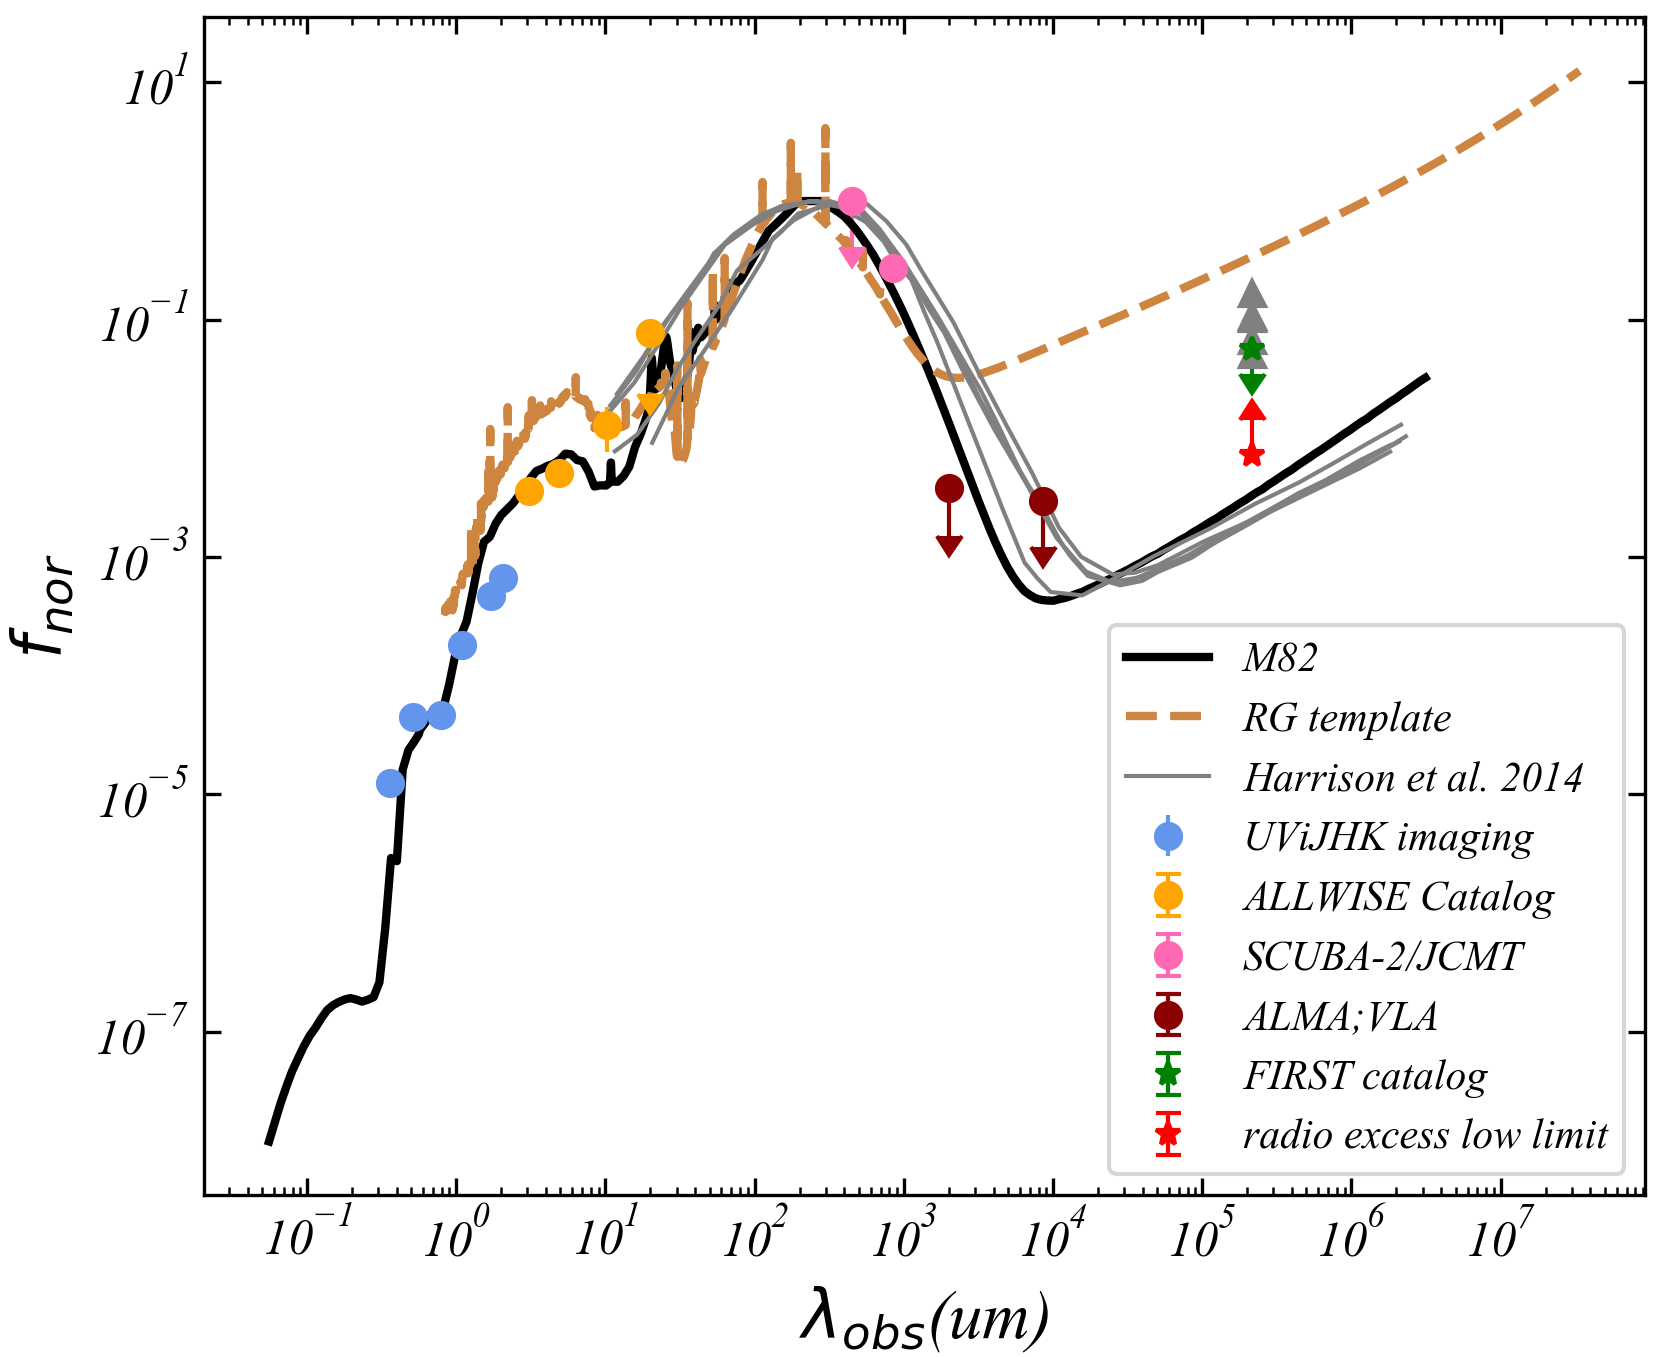
\includegraphics[width=\columnwidth]{figs/SED_fitting}
		\label{SED}
	\end{figure}
	
	We use the definition given by \cite{ivison2010far} to calculate the ratio between the far-infrared ($\rm 8-1000 \ \mu m$) and radio emission ($\rm q_{IR}$), this ratio is usually used to identify if there is significant radio emission above that expected from their star-formation activity (radio emission results from AGN or other process). The formula is given by:
	\begin{equation}
		\rm q_{IR}=log[\frac{S_{IR}/3.75 \times 10^{12} W \ m^{-2}}{S_{1.4}/W \ m^{-2} Hz^{-1}}]
		\label{q_IR}
	\end{equation}
	where $\rm S_{IR}$ is the rest-frame flux in far-infrared range ($8-1000 \ \rm \mu m $) and $\rm S_{1.4}$ is the rest-frame 1.4 GHz flux density. \citep{arrigoni2018overdensity} performed a follow-up observation for MAMMOTH-1 and constrain the SED with the available data. They found the SED of local starburst galaxy M82 match significantly well with the observations which indicates that BOSS1441 is possibly an Ultra-Luminous Infrared Galaxy (ULIG). The far-infrared luminosity is then integrated from this SED $\rm L_{IR}=3.2 \times 10^{12}L_{\odot}$. Through setting the luminosity distance to be $\rm D_{L}=18773.8$ Mpc at redshift z=2.3, it is easy to calculate the far-infrared flux $\rm S_{IR}=2.9 \times 10^{-16}\ W \ cm^{-2}$.  Because the D-configuration of VLA doesn't cover $\rm \nu_{obs}=0.42$ GHz (1.4 GHz in rest frame), we adopt $\rm S_{1.4}$=0.01 mJy from M82 SED template. We note here that the constrain of continuum, $f_{150,up}$, is one-order-magnitude lower than that of M82 SED template, therefore the true flux density at $\rm \nu_{rest}=1.4$GHz should be lower than 0.01 mJy. By adopting $\rm S_{1.4}=0.01 mJy$ the low limit of $\rm q_{IR}$ is equal to 1.9. \cite{ivison2010far} and \cite{del2013goods} define "radio excess" sources as those with $\rm q_{IR} \leqslant 1.8$, according to this definition and $\rm q_{IR}$ calculated here, we suggest BOSS1441 is a radio-quiet source with no significant continuum radio emission.

\subsection{Morphology and Emission}

We construct continuum-free line images by summing over the wavelength range of the emission lines in data cubes and subtracting the underlying continuum component from them. The continuum component is estimated by taking average from another wavelength range out of line emission ( or absorption). We show the results in the left panel of Fig. \ref{overlayspec}. The three contours of different colors representing signal-to-noise ratio (SNR) show the spatially extended emission of Ly$\alpha$ HeII and CIV with the first contour corresponding to 2 and steps between contours to 2. The background image was taken by Wide Field Camera 3 (WFC3) on Hubble Space Telescope (HST) with F160W filter. Sources labeled from G-1 to G-5 are galaxies at the same redshift ($\rm z \approx 2.3$) with Source-B confirmed by CO (1-0) emission and CO (3-2) emission \citep{emonts2019cold,qiongli2020}. The emitting structure shows Ly$\alpha$ nebula covers all of the marked objects and extends to $\rm 20\arcsec$ which corresponds to 164 kpc. It also shows that the physical projected size of extended HeII and CIV emission reaches to $9 \arcsec$ corresponding to 74 kpc.

Spectra are extracted within aperture centering on the peak of emission with radius of $1.5\arcsec$ (larger than the spatial resolution of KCWI) and shown in the right panel. To determine the redshifts of these widely extended nebulaes, we fit the three emission lines with one-component gaussian function and estimate the wavelength of line centre. The fitted parameters are shown in Tab.\ref{fit_L}. By converting the line width (\AA) to FWHM (km/s) it seems that all of the three emission line have a relatively large FWHM which equals to $\rm FWHM_{Ly}=1225 \ km/s$, $\rm FWHM_{HeII}=1039 \ km/s$ and $\rm FWHM_{CIV}=1786 \ km/s$. This result indicates that there may be extremely violent kinematic activity in the nebula on a physical scale of 100 kpc.

Because the surface brightness (SB) values for both kinematically narrow and broad features would have been either lost in the noise or underestimated in a narrow-band (NB) image with single width of wavelength, we adopt optimally-extract method from \citet{borisova2016ubiquitous} to construct psudo-NB images which can reach to a larger dynamic range comparing to a standard image. These images are obtained by using a three dimensional segmentation mask (3D mask) which defines a three-dimensional SNR surface in the cube, pixels with values below the SNR threshold are masked and only pixels possessing significant signal are extracted. Therefore, the signal of each pixel are integrated along a slightly different range in wavelength which allows us to obtain images or spectra with maximal SNR after stacking along spatial axis or spectral axis. In particular, images presented in Fig. \ref{kinematicsmap} (left column) are obtained by using this method after continuum-subtraction and stacking along spectral axis. The three extended emissions are detected at faint levels with 1-$\sigma$ SB of $\rm SB_{Ly}=xxx \ erg \ s^{-1} \ cm^{-2} \ arcsec^{-2}$, $\rm SB_{HeII}=xxx \ erg \ s^{-1} \ cm^{-2} \ arcsec^{-2}$ and $\rm SB_{CIV}=xxx \ erg \ s^{-1} \ cm^{-2} \ arcsec^{-2}$. 


\begin{figure*}
		\centering
		\subfloat[contour]{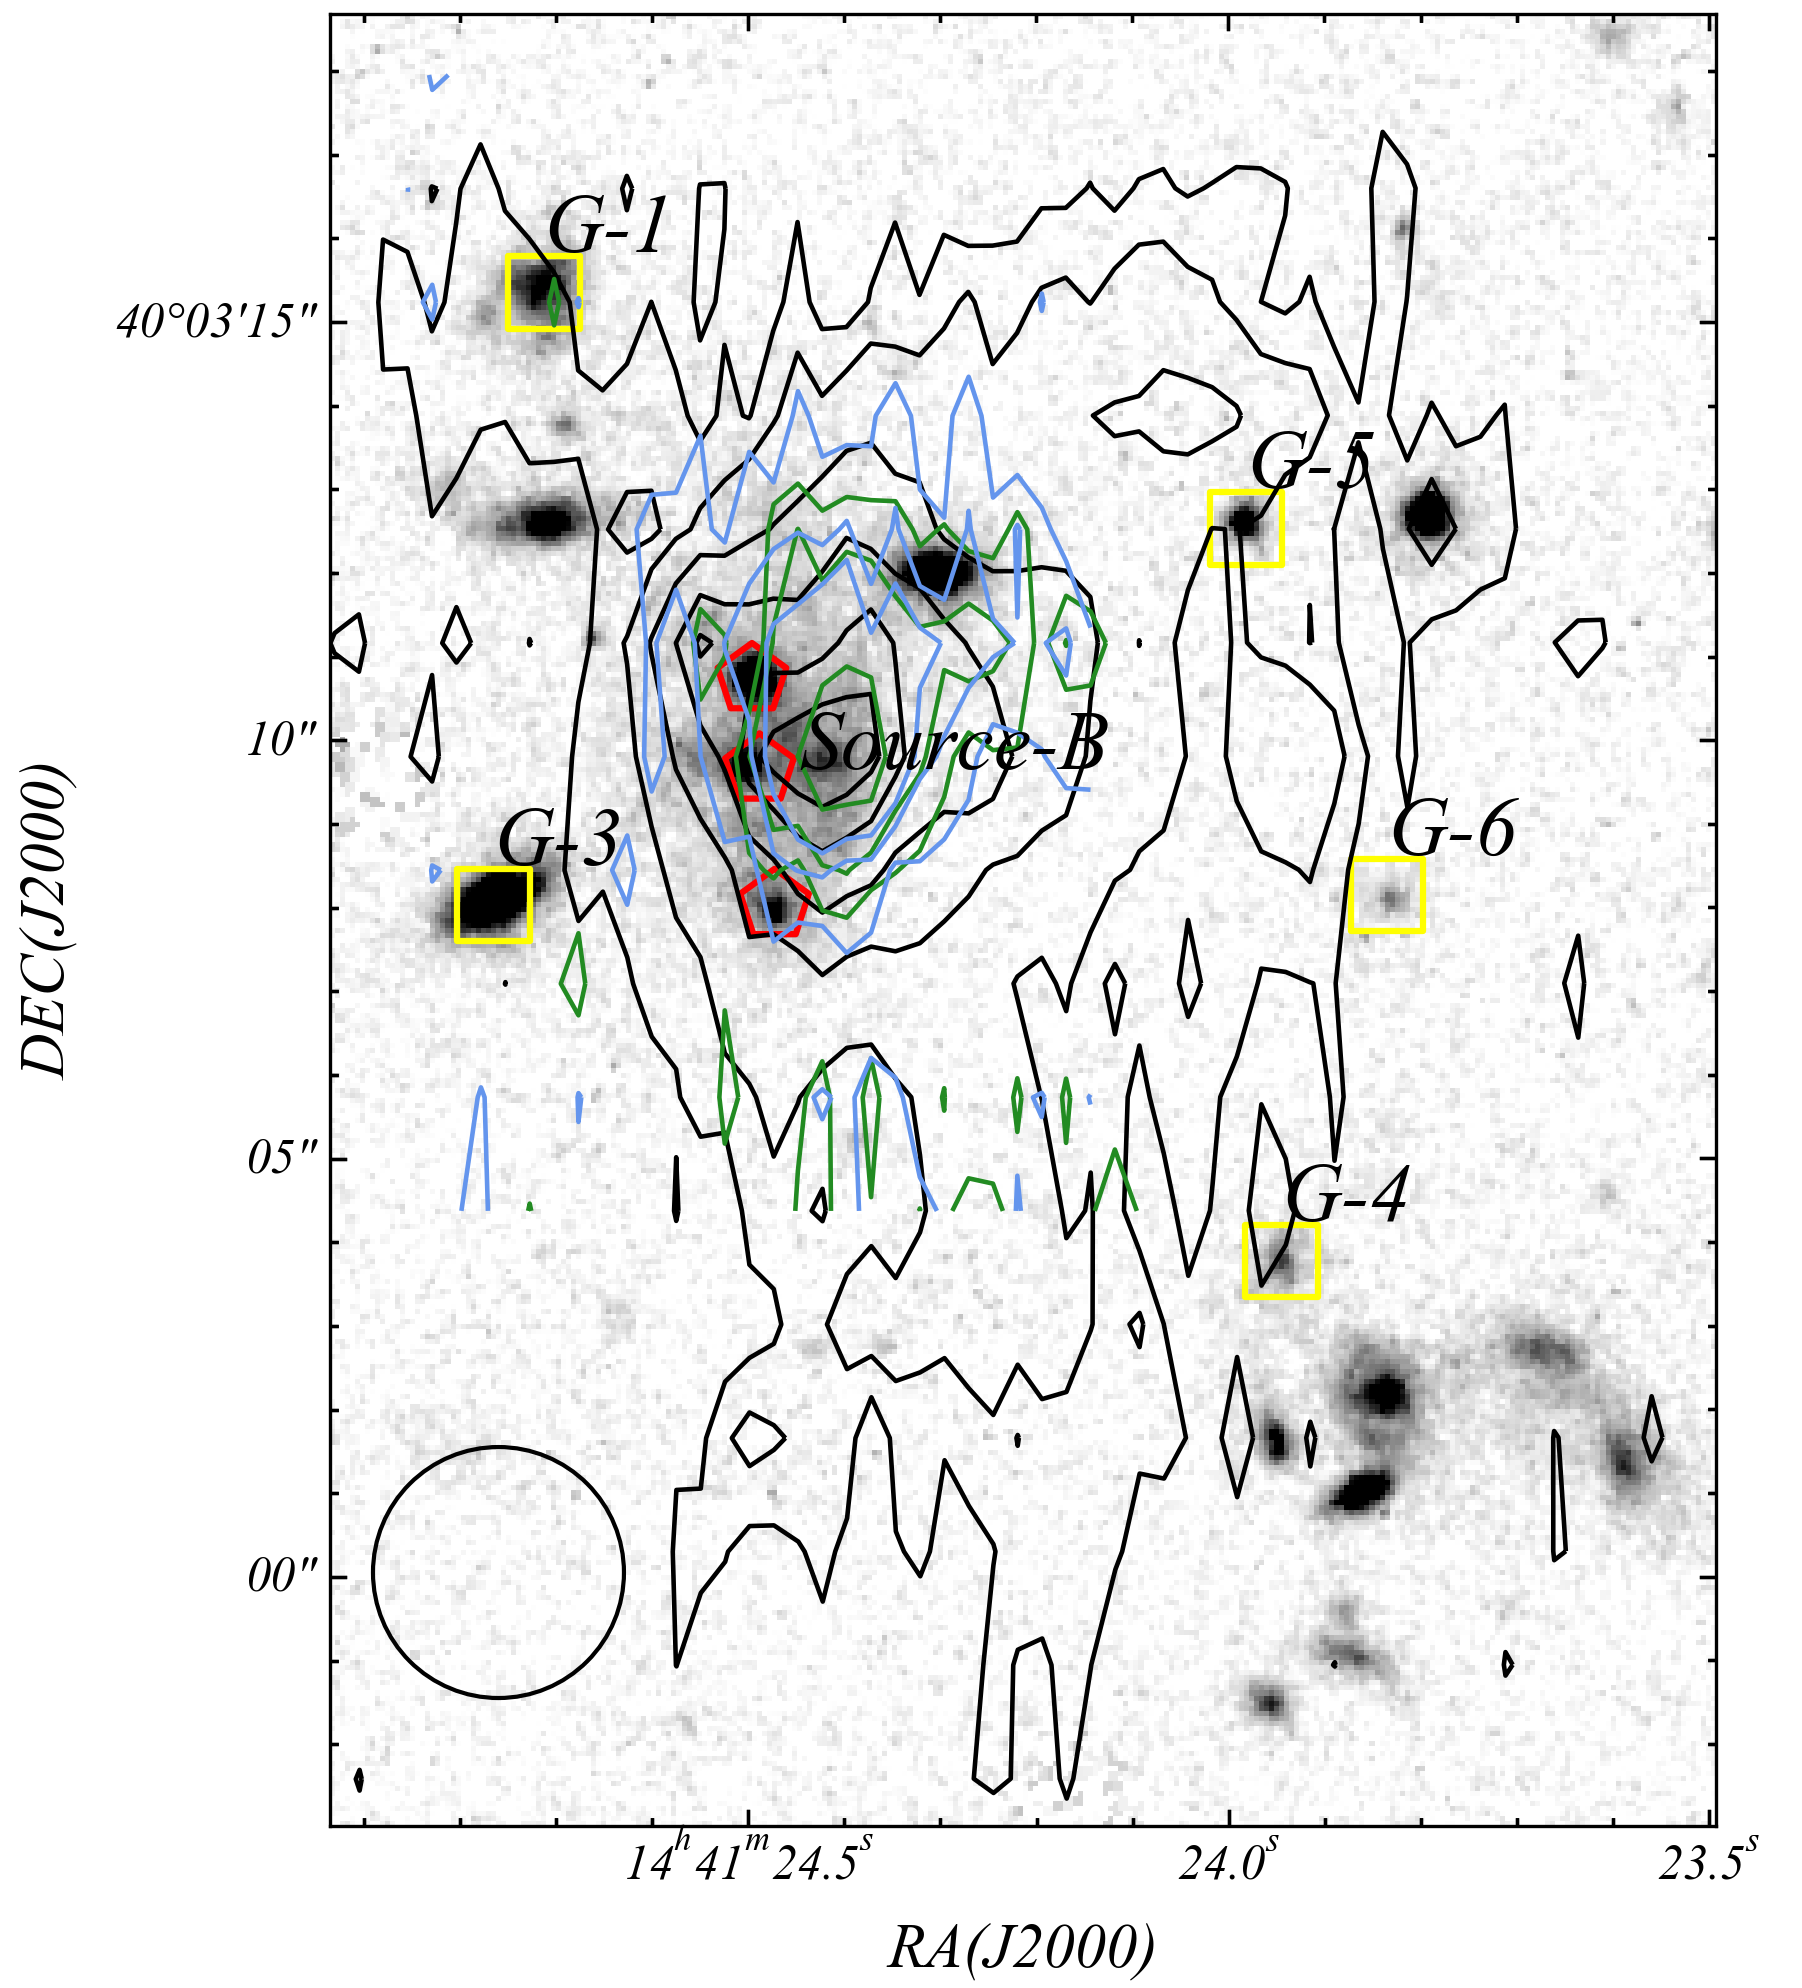
\includegraphics[width=0.5\textwidth]{figs/contour}}
		\subfloat[spectra]{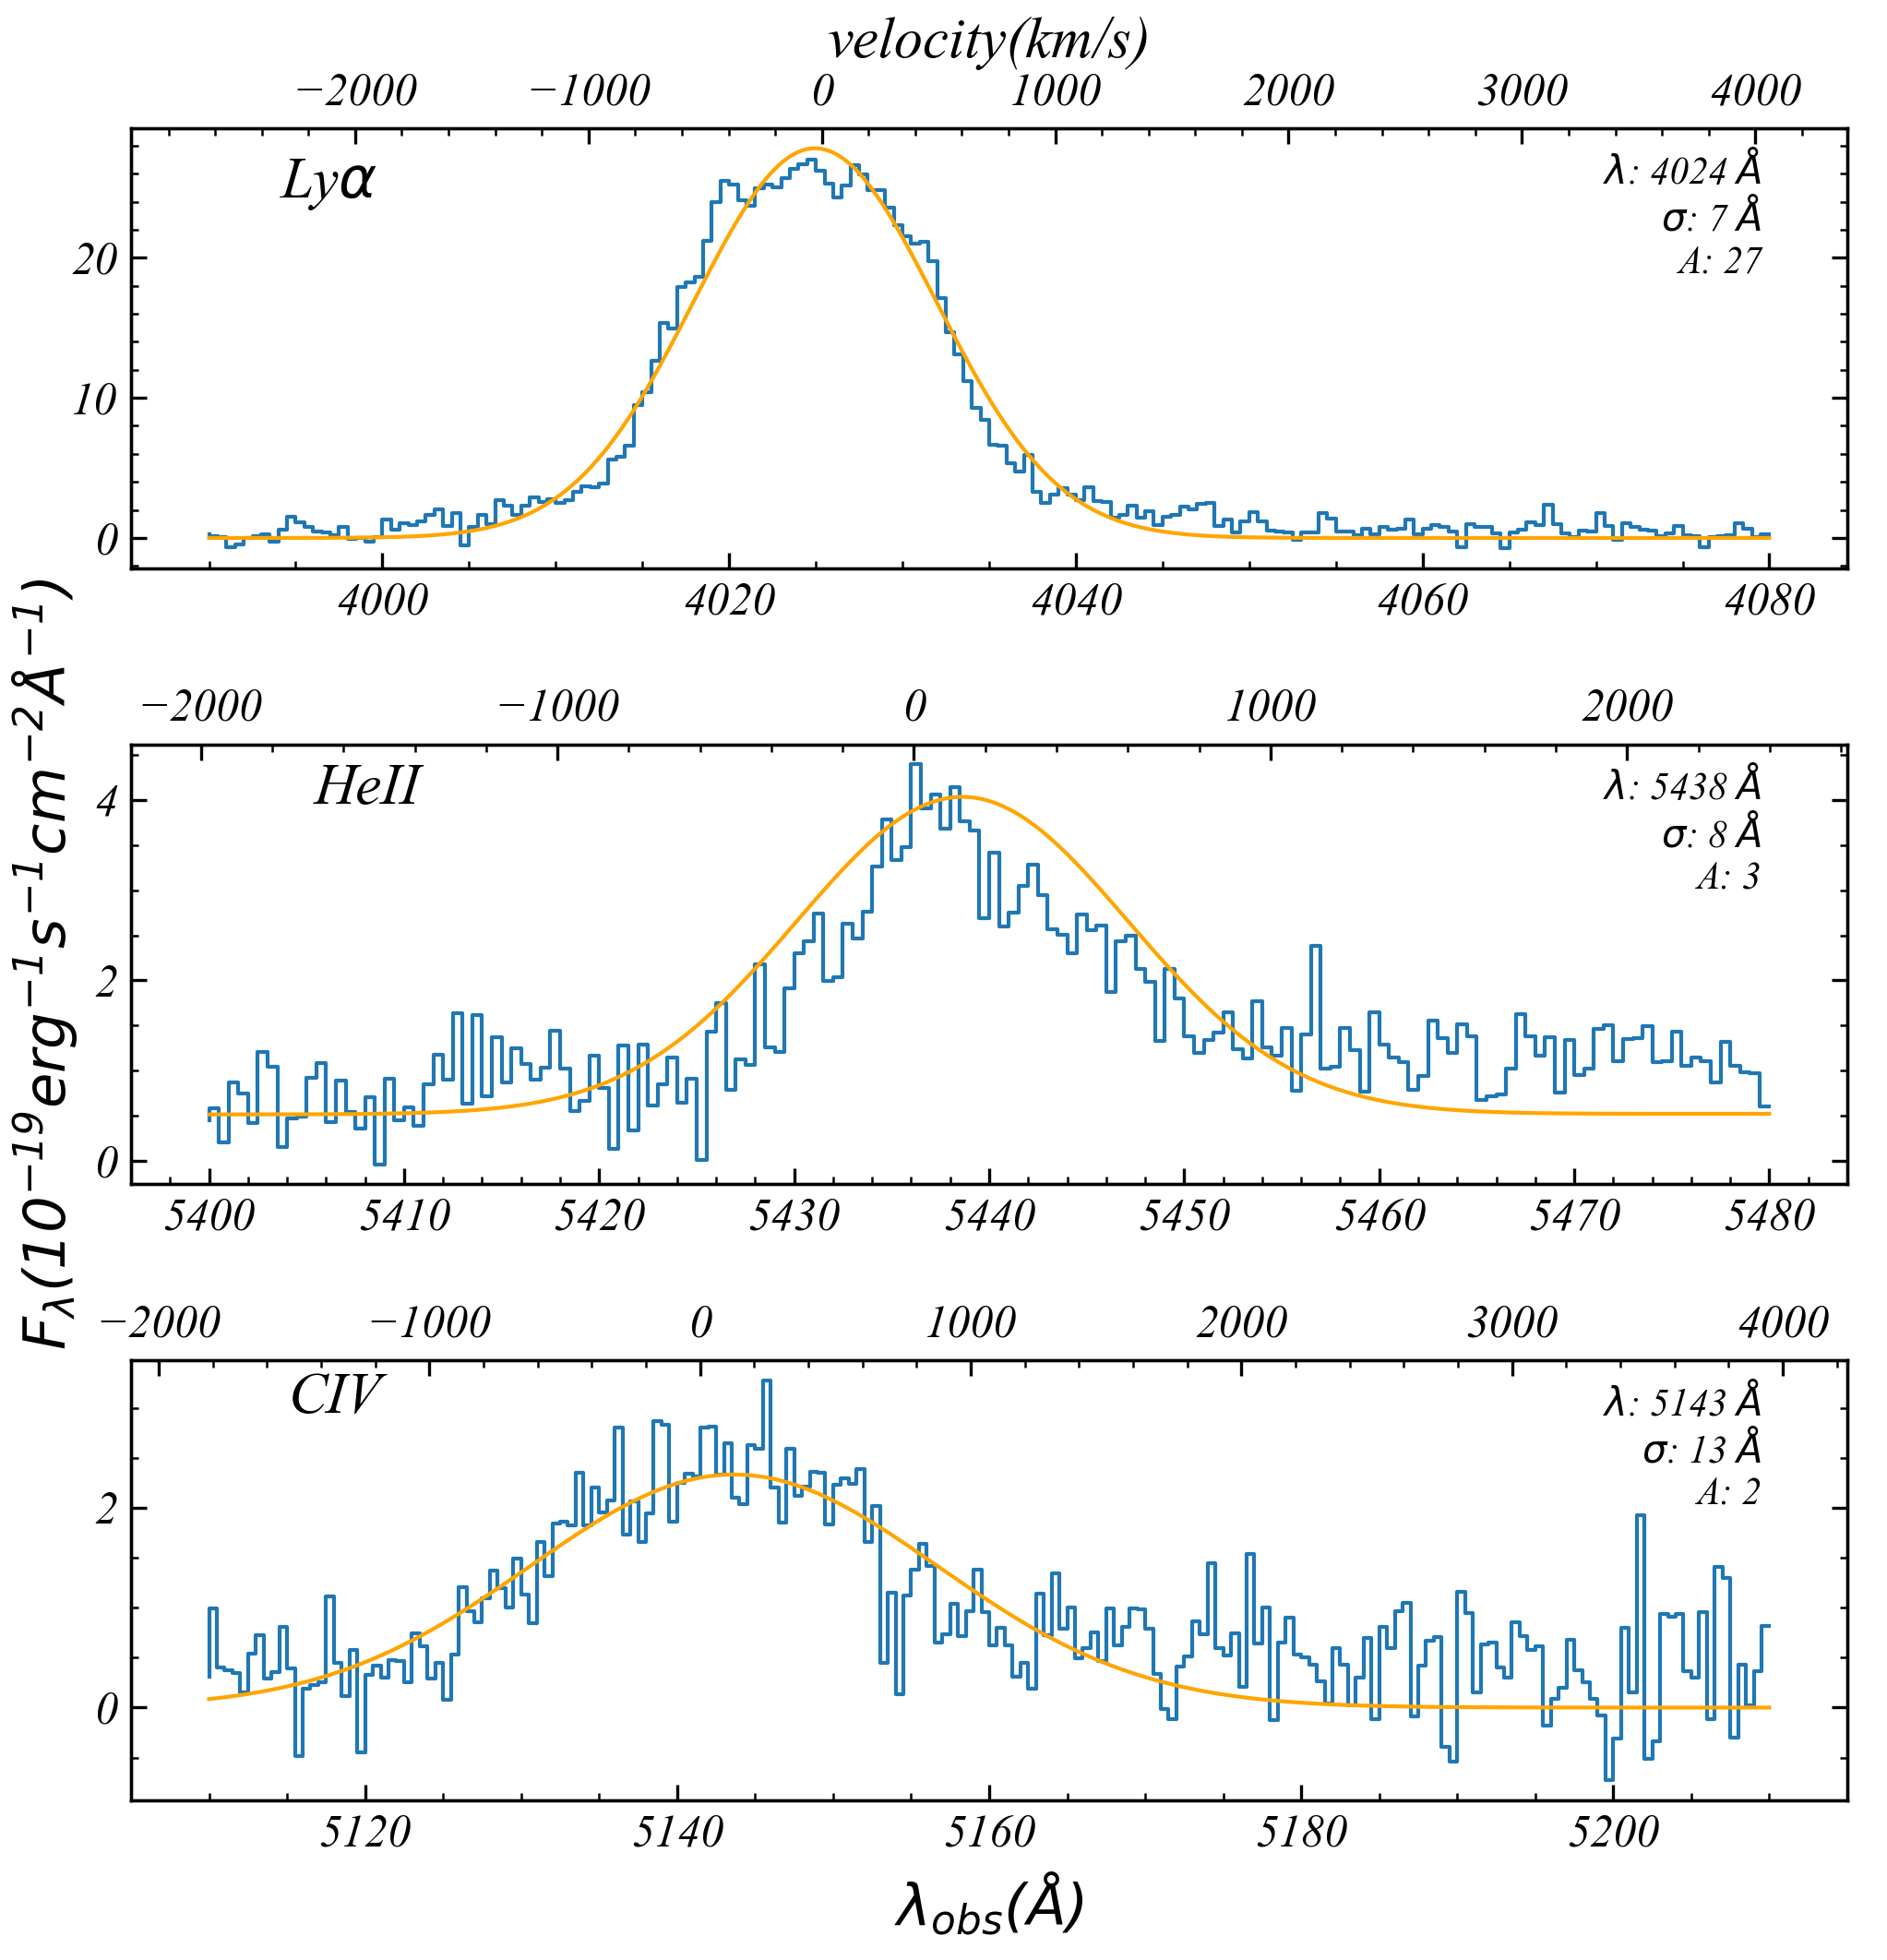
\includegraphics[width=0.5\textwidth]{figs/spectral}}
		\label{overlayspec}
		\caption{Left: HST image of MAMMOTH-1 from circle 24,25, PI: Cai. We overlay on it Ly$\alpha$ HeII and CIV psudo narrow band images. Black contour is Ly$\alpha$, blue contour is HeII, green contour is CIV. We also mark source-B with red mark and sources at the same redshift with yellow mark. We also plot circle with raidus of 1$arcsec^{2}$. Right: spectra of the 3 emission lines extracted from aperture center on source-B with radius 1$arcsec^{2}$, we fit them with one-component gaussian function.}
\end{figure*}
	\begin{table}[htp]
	\begin{center}
		\begin{tabular}{ccccc}
\hline
\hline
& $\rm \lambda_{c}$(\AA) & $\rm \sigma_{\lambda}$(\AA) & L(erg/s) & redshift \\ \hline
Ly$\alpha$ &   4024  &     7  &   $\rm 2.68 \times 10^{44}$ & 2.310        \\
HeII       &   5438  &     8  &   $\rm 1.97 \times 10^{43}$ & 2.316        \\
CIV        &   5143  &     13 &   $\rm 2.29 \times 10^{43}$ & 2.320        \\ \hline
\end{tabular}
\end{center}
	\caption{}
	\label{fit_L}
	\end{table}

\subsection{Kinematics}

In this section we present the maps for flux-weighted velocity and flux-weighted dispersion of Ly$\rm \alpha$, HeII and CIV emissions produced with the 3D mask to get an indication of kinematic patterns. We note that Ly$\rm \alpha$ resonant scattering effect doesn't play an important role on kinematics seen in the central area because it tends to disrupt the coherency of kinematics instead of enhancing it \citep{Cantalupo2005Fluorescent}, this is also confirmed by the results of HeII and CIV emissions.

Fig. \ref{kinematicsmap} shows the two moment maps together with the optimally-extracted images of the three emissions. The optimally-extracted images in left panel clearly shows the projected physical scale of Ly$\rm \alpha$ emission extends to 175 kpc which approximates the typical size of dark matter halo at this redshift. This projected scale is smaller comparing to the results of \citet{cai2017discovery} due to small FoV ($\rm 20\arcsec \times 33\arcsec$) of KCWI. In addition, HeII and CIV emission also extends to tens of kiloparcsec surpassing the typical size of galaxies, especially CIV emission which extends to 88 kpc. This spatially widely extended metal emissions are rarely seen at high redshift with such large projected scale.

In the middle and right panel we present the maps of first and second moment of flux distribution. The middle panel represents the flux-weighted centroid velocity maps, it shows that the velocity gradients are evident in the three maps with same direction from the northwest to the southeast. This kinematic pattern is usually the indication of rotating gas disk in CGM or outflow ejected from central AGN. Besides, the velocity map of Ly$\rm \alpha$ emission also shows gradient around G-5 from northeast to southwest.  The velocity dispersion map of Ly$\rm \alpha$ emission shows that the area around source-B possesses larger velocity dispersion ($\rm \sigma_{v} > 400 \ km/s$) and extends to $\rm 100 \ kpc$, dispersion even larger than 650 km/s which corresponds to FWHM of 1550 km/s in some spatial positions. Following the same method in \citet{Arrigoni_Battaia_2018} the expected velocity dispersion calculated for a dark matter halo hosting quasars is 300 km/s with the results $\rm M_{DM} \approx 10^{15.2} \ M_{\odot}$ in \citet{arrigoni2018overdensity} where $M_{DM}$ is the mass of dark matter halo. The significant comparison between expected dispersion and our results may indicate that there is extremely powerful kinematic activity in this region which is impossibly caused by rotation or inflow.

Fig. \ref{slices} shows the channel map of Ly$\rm \alpha$ emission with step of 200 km/s. It is clearly seen that the red component and blue component are on either side of source-B. Besides, We also extract the spectra which are normalized and fitted with one-component gaussian function of different spatial positions from circular aperture with radius of $\rm 1.5 \arcsec$ and show it in Fig. \ref{spectralss}. No significant symmetric doublets existing in the spectra confirms that the resonant scattering effect is negligible. 

Based on the above analysis, we rule out the possibility that the kinematic pattern is result from rotating gas disk, inflow and resonant scattering effect of Ly$\rm \alpha$ emission. Together with the existing of extended HeII CIV and OIII emission \citep{cai2017discovery}, the most natural and straightforward interpretation is that there is extremely powerful and widely influenced outflow ejected from source-B which has the ability to influence the entire gas environment in dark matter halo hosting source-B. The large-scale feedback effect has been widely reported before, however these observations mainly focus on the central galaxies of low redshift clusters and they are mostly powered by jet with significant radio signal. So, the halo-scale-influenced outflow with no strong radio signal at high redshift makes our observation extremely unique. So understanding the mechanism powering this strong outflow in our observation is essential for feedback effect on galaxy evolution.  

	 \begin{figure*}[htp]
		\centering
		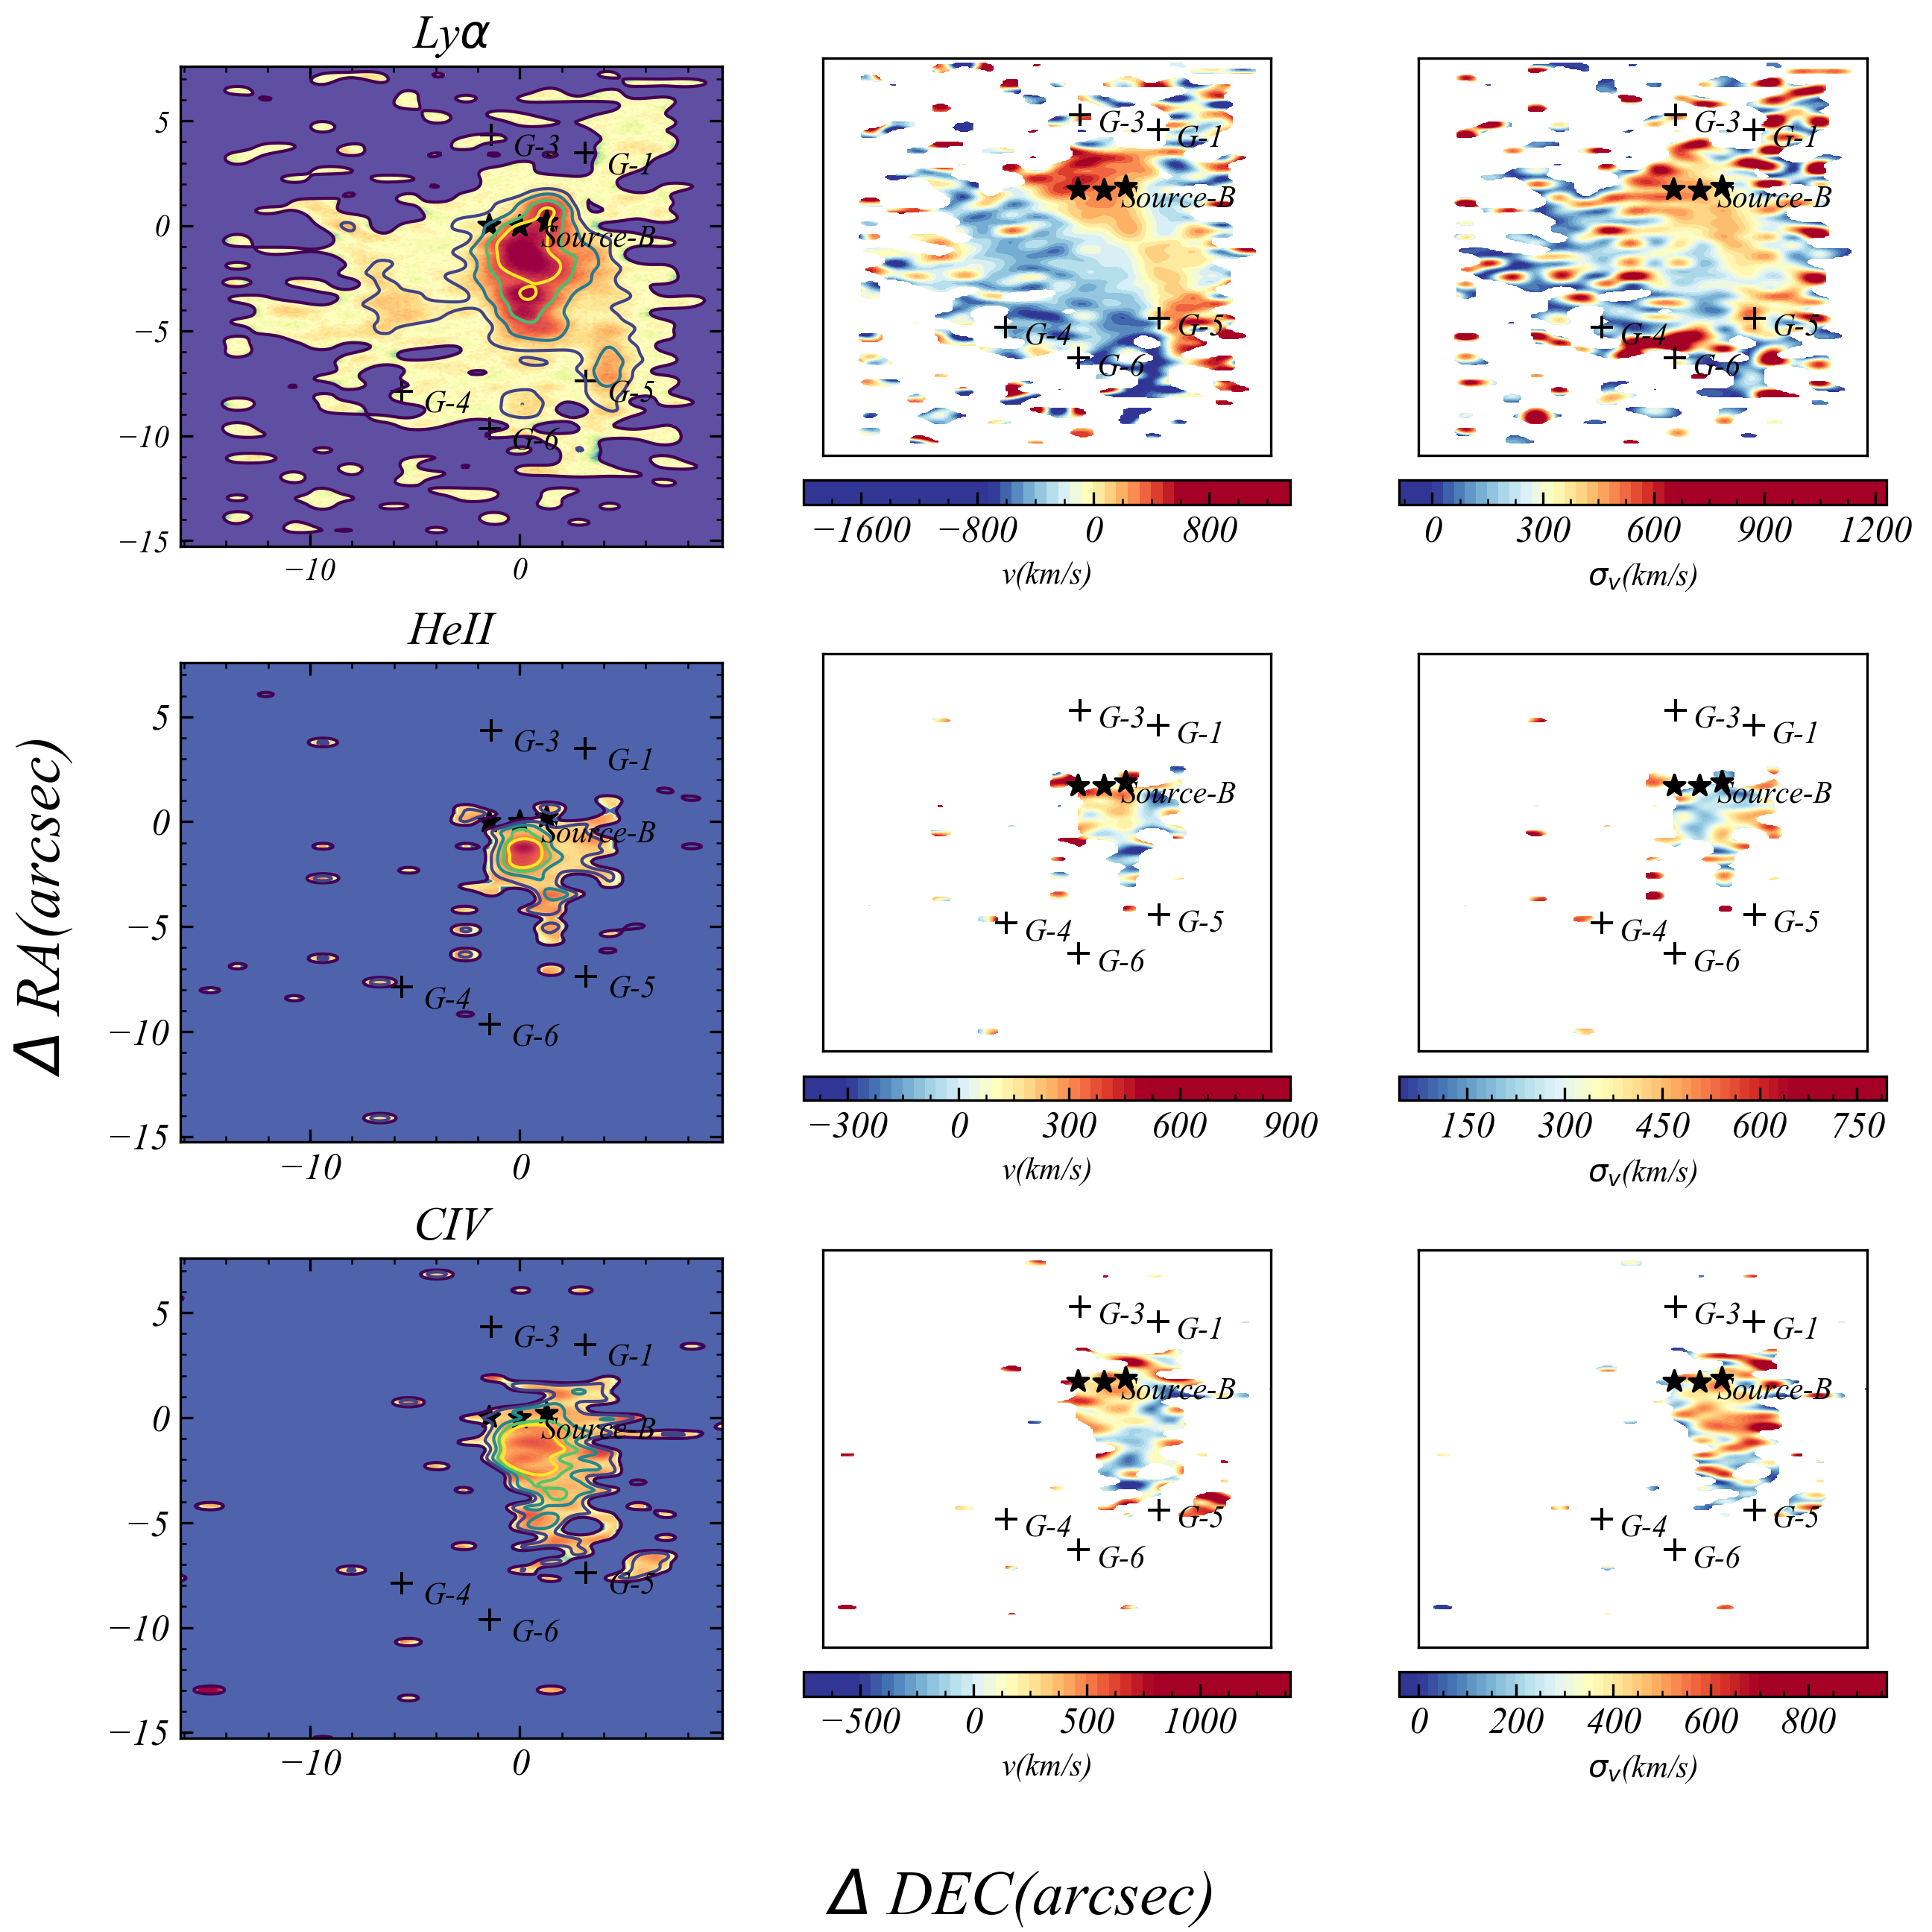
\includegraphics[width=\textwidth]{figs/emissionmap}
		\label{kinematicsmap}
		\caption{Left: continuum-subtracted psudo-narrow band images for the 3 emissions. We select regions $> 1.5\sigma$ in each slice and stack these slices together. The contour represent signal-to-noise ratio(SNR), for ly$\alpha$ is ($5\sigma,9\sigma,18\sigma,30\sigma,42\sigma,51\sigma$), for HeII is ($3\sigma,5,9\sigma$) and for CIV is ($4\sigma,7\sigma,9\sigma$). Middle: flux-weighted velocity map with respect to the systemic redshift of MAMMOTH-1. Right: flux-weighted velocity dispersion also with respect to systemic redshift of MAMMOTH-1. We also mark sources in the field with cross.}
	\end{figure*}
	
	\begin{figure*}[htp]
		\centering
		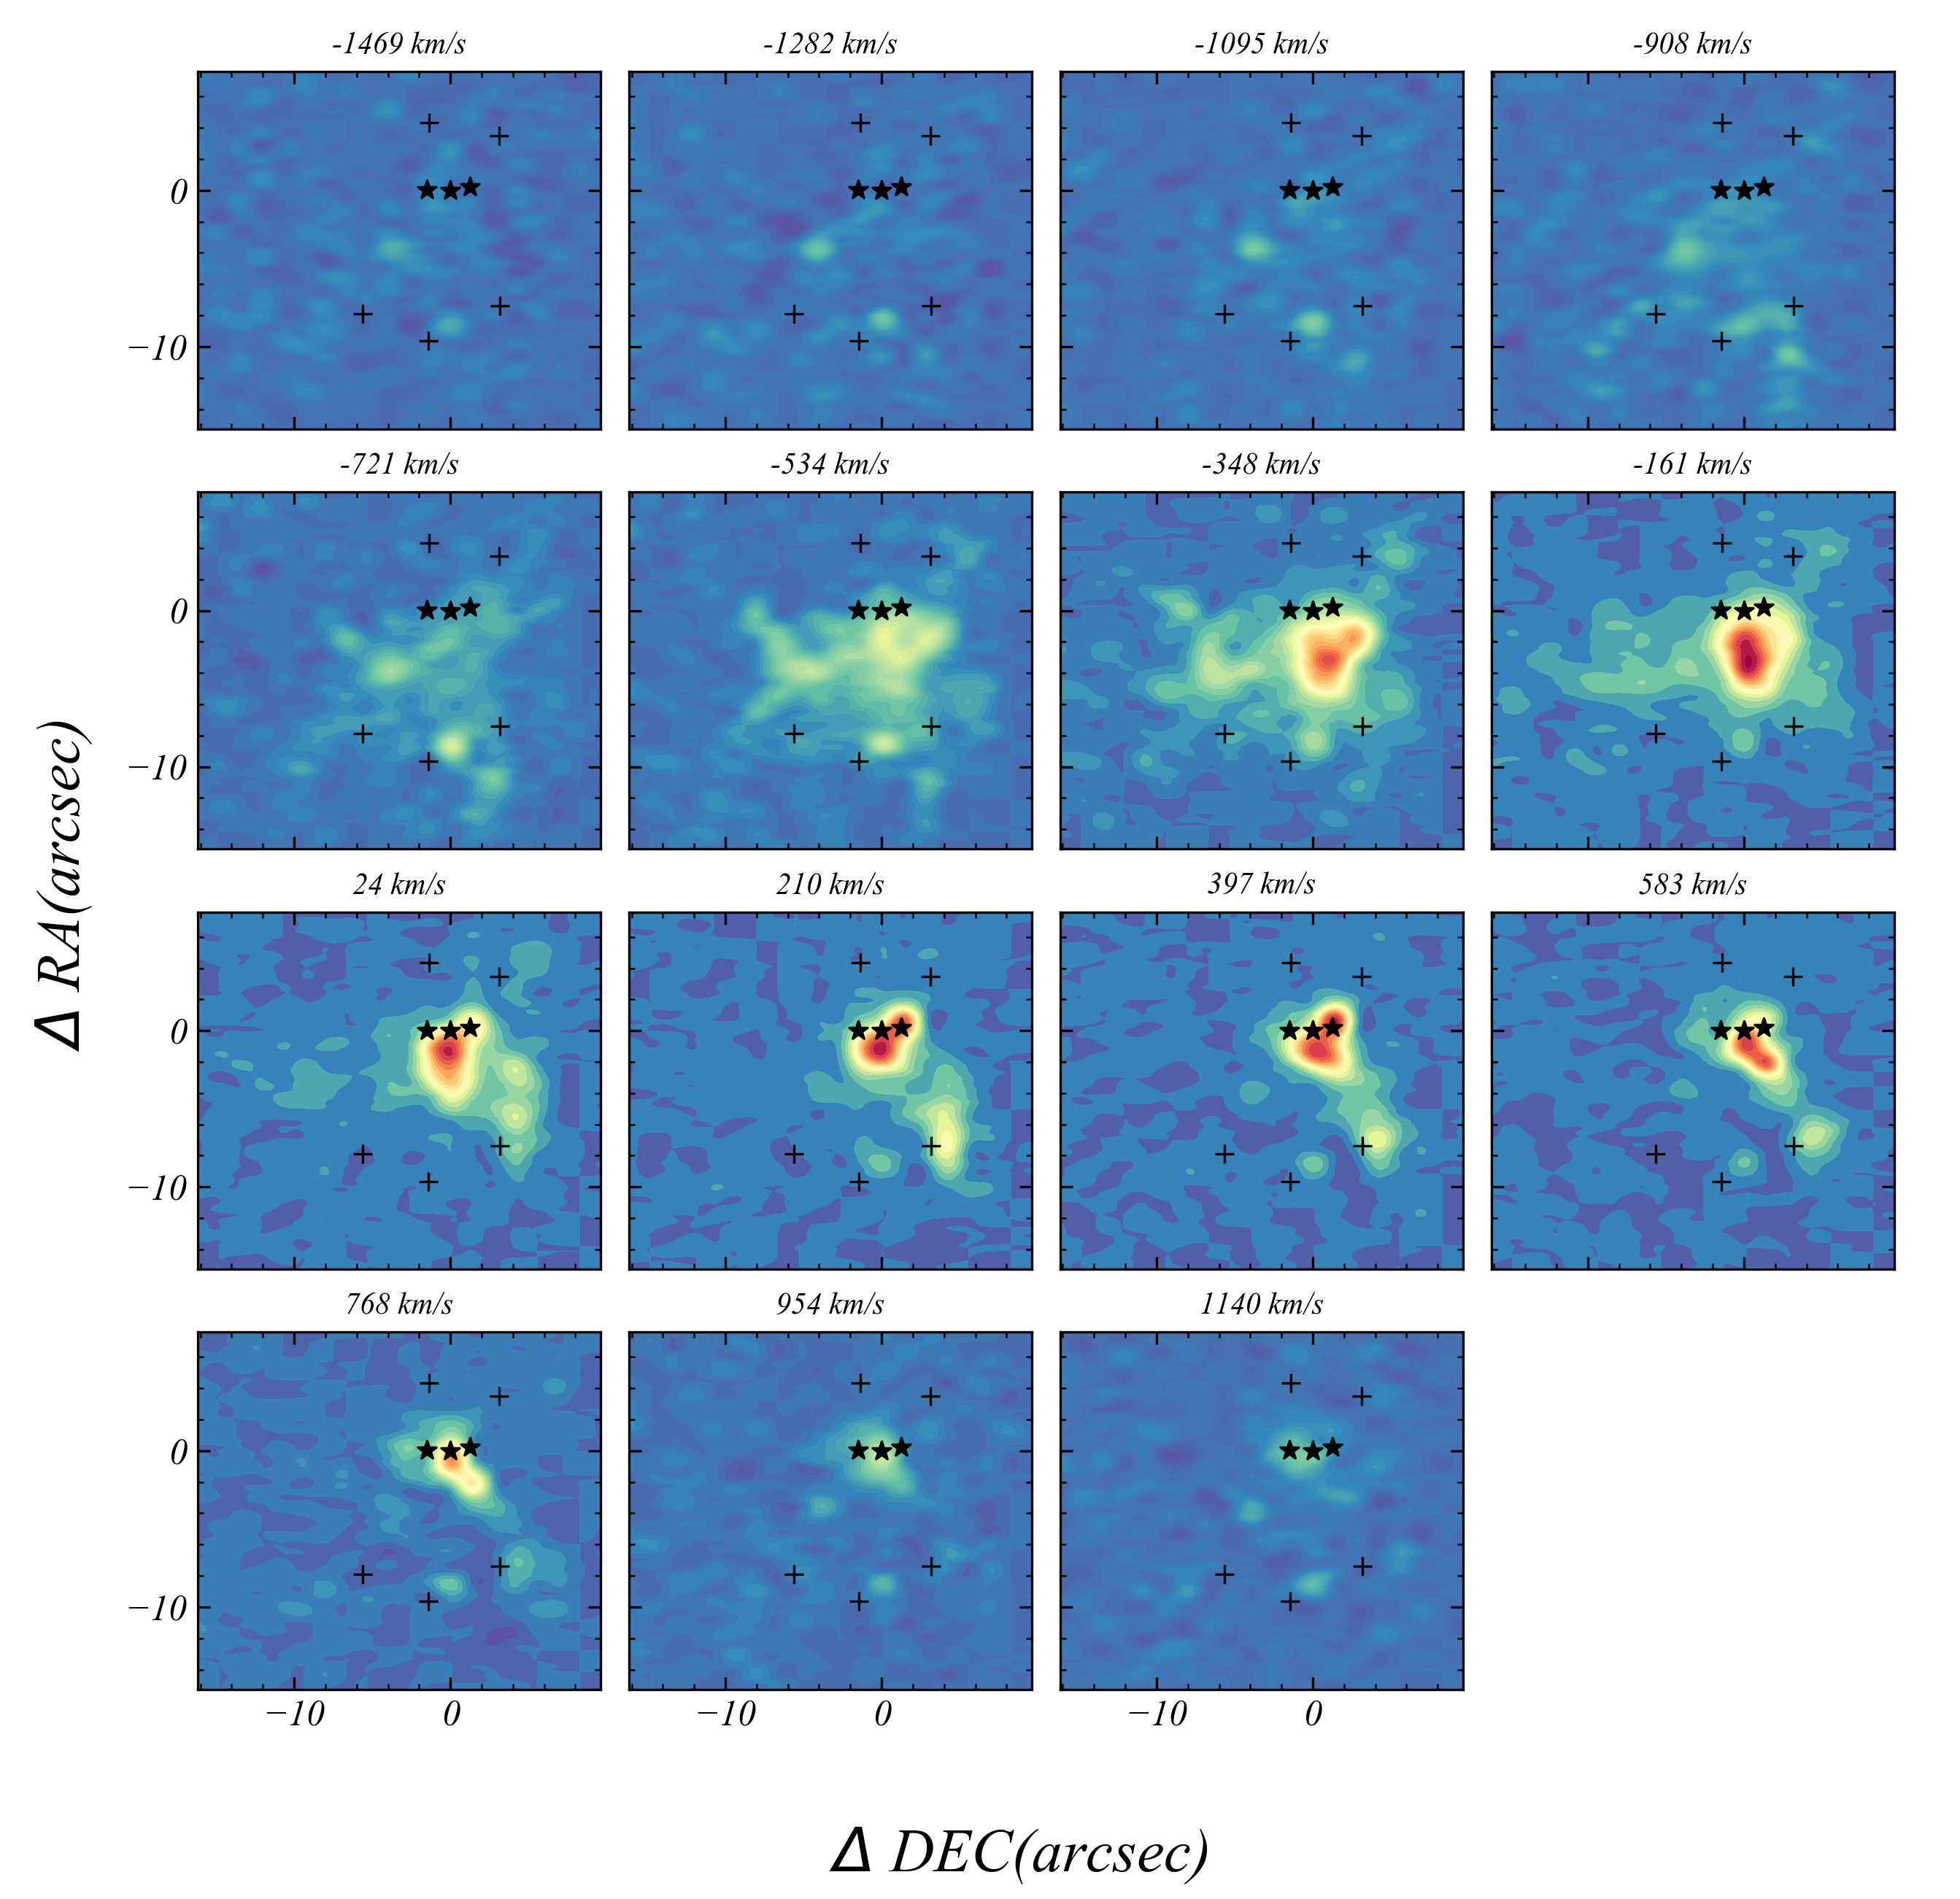
\includegraphics[width=\textwidth]{figs/slices}
		\label{slices}
		\caption{Kinematics of cool gas. It shows signal of ly$\alpha$ emission at different velocities. We select $\Delta v=187$km/s which corresponds 4$A$  as the bin size of these slices. We extract these slices within the range $4000A-4040A$, for each image here, we use the mean velocity of the bin as title for each image. It shows significant red and blue component on either side of source-B.}
	\end{figure*}
	
	\begin{figure*}[htp]
		\centering
		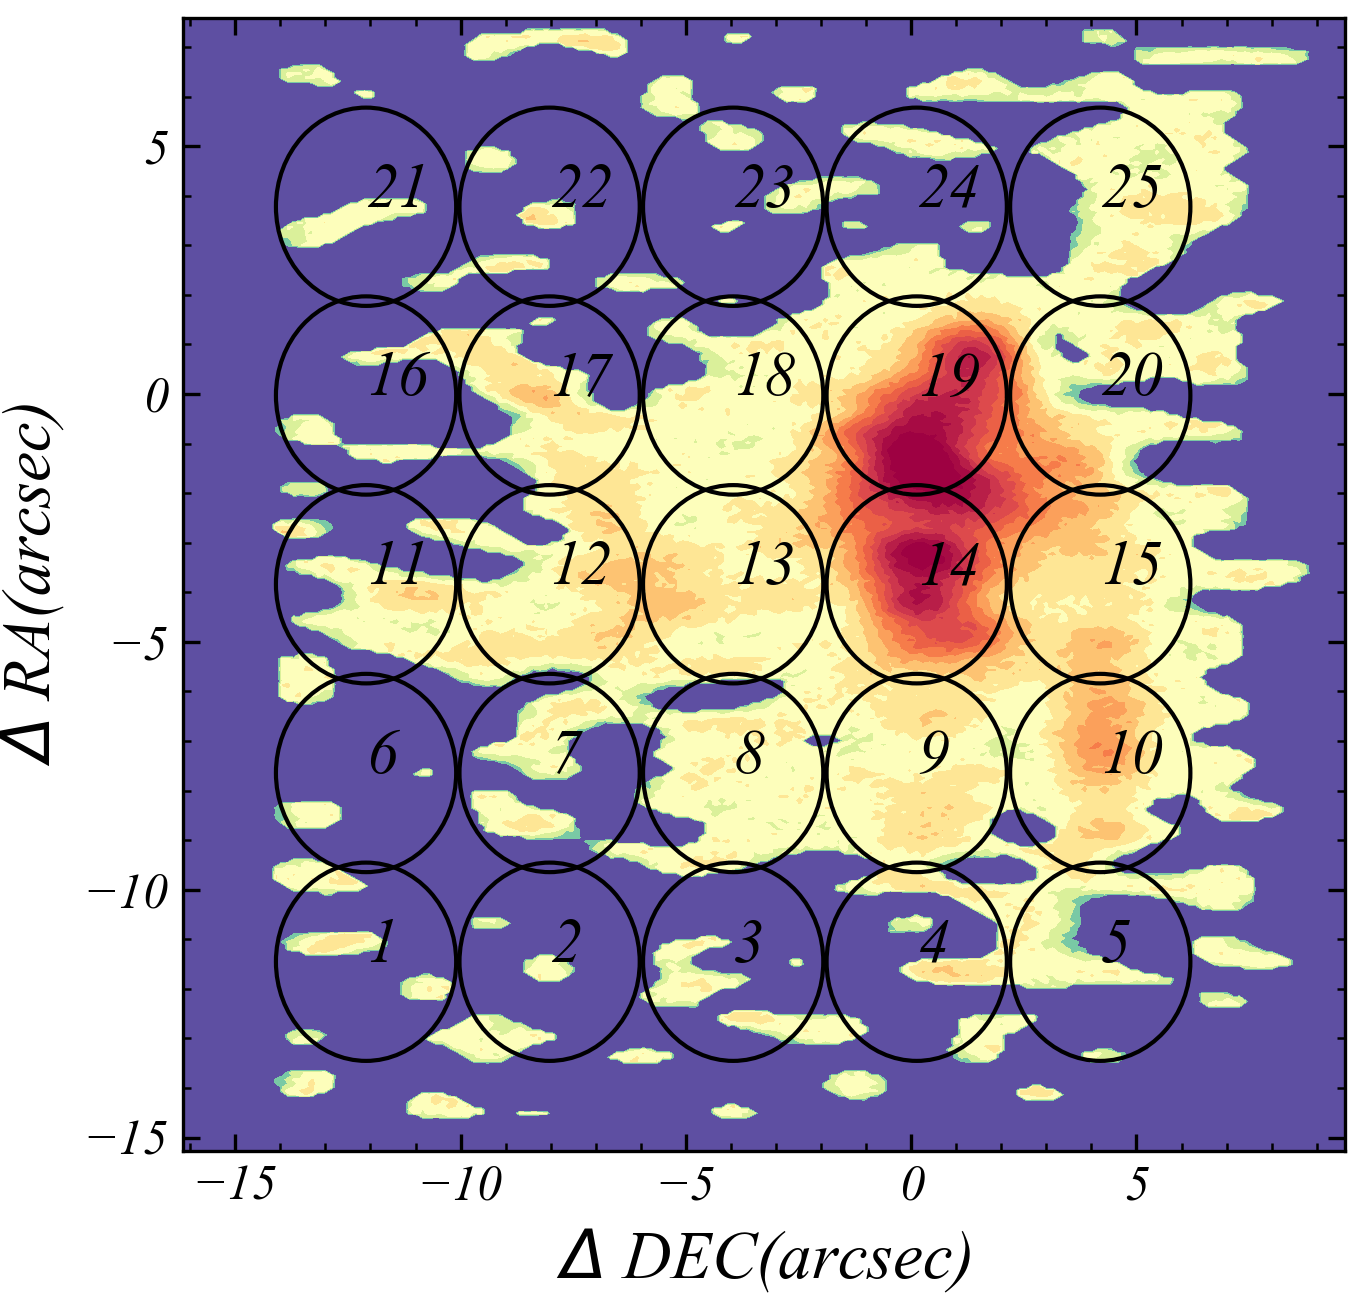
\includegraphics[width=0.5\textwidth]{figs/apertmap.png}
	\end{figure*}
	\begin{figure*}[htp]
		\centering
		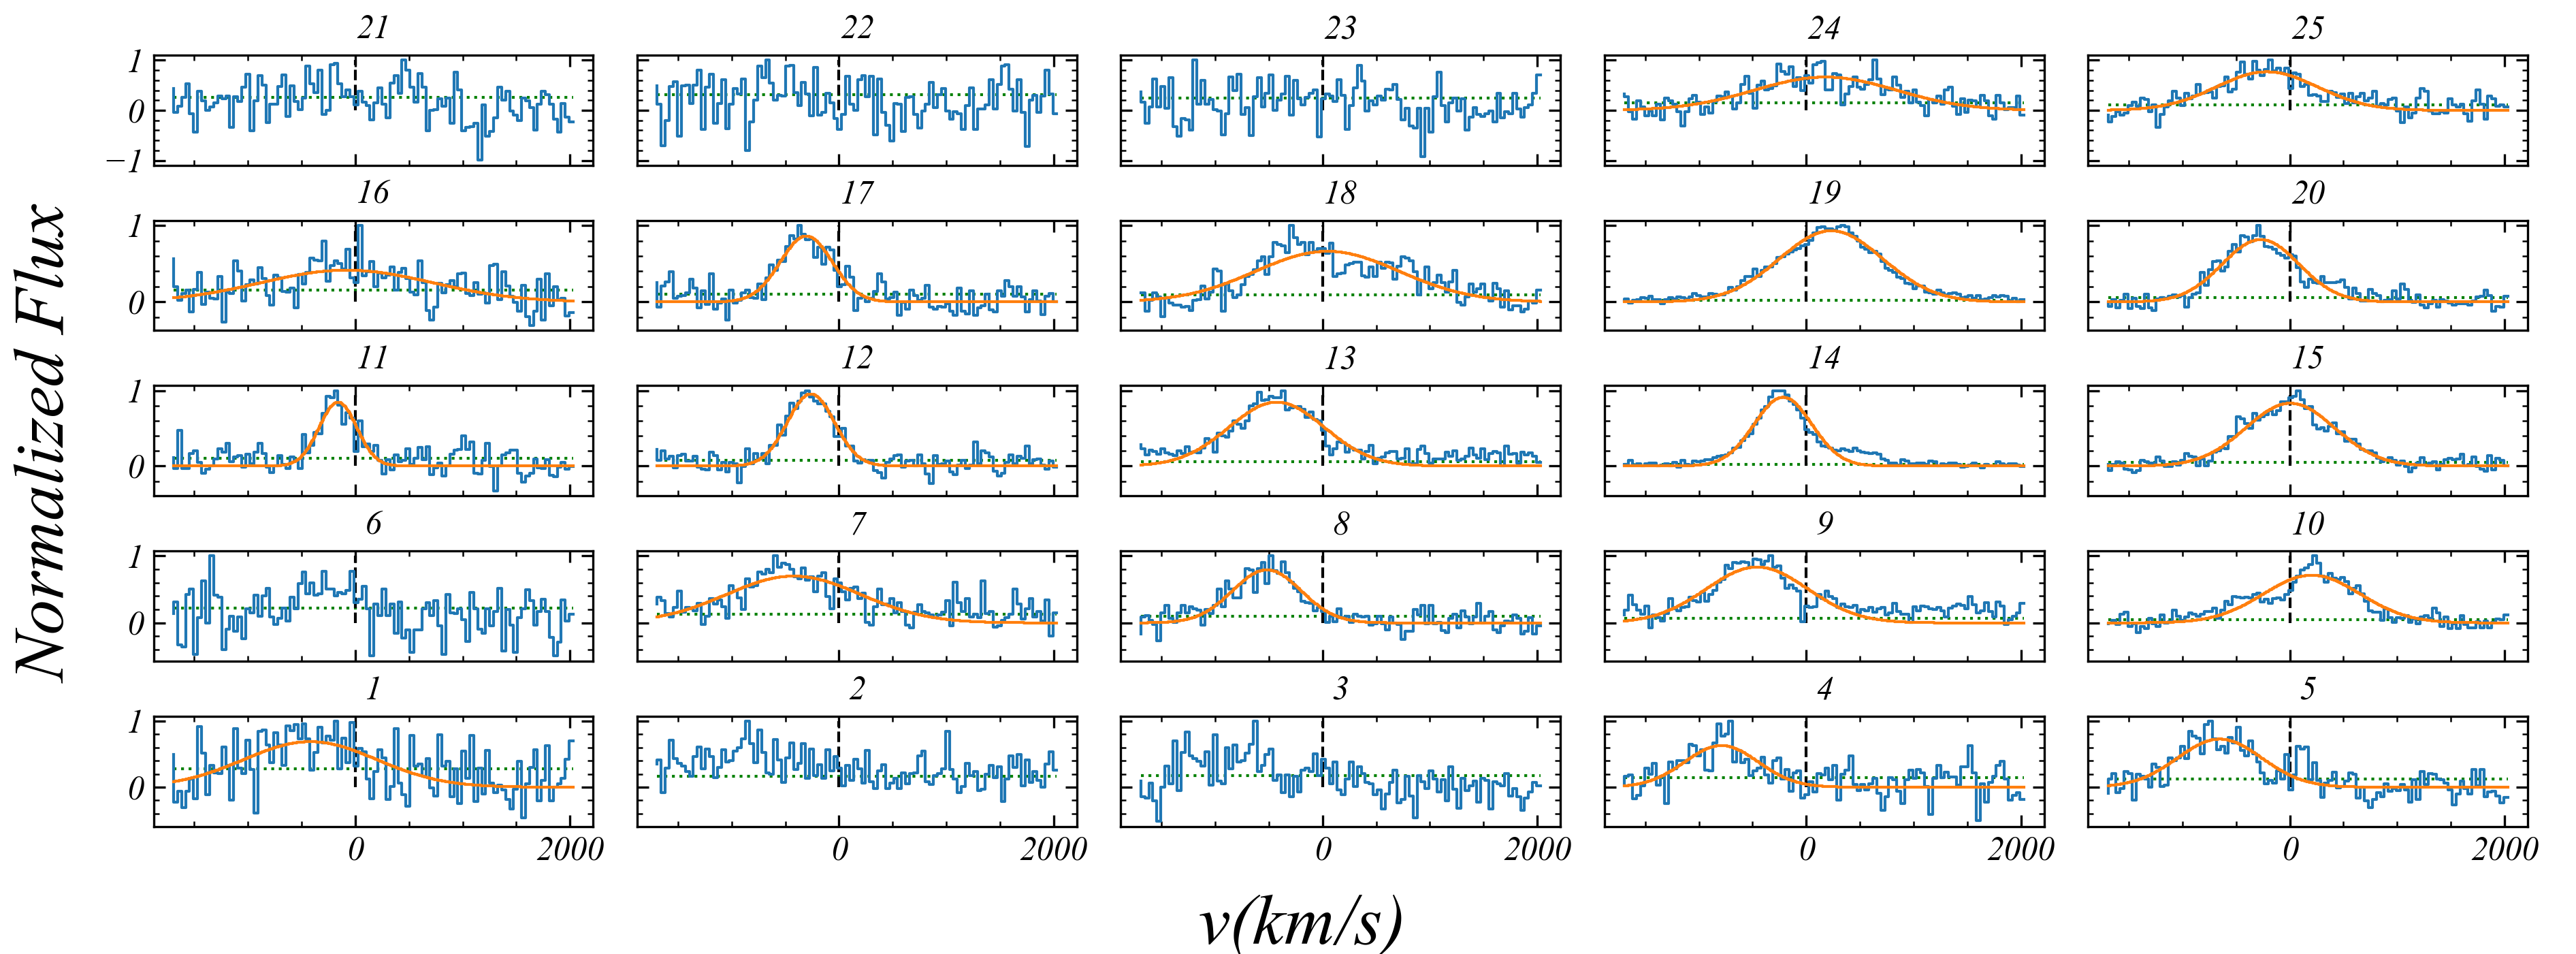
\includegraphics[width=\textwidth,height=0.45\textwidth]{figs/specmap}
		\label{spectralss}
		\caption{Up: Continuum-subtracted psudo narrow band image of ly$\alpha$. We overlay circles on it and number them from 1 to 25.  Low: Continuum-subtracted spectra extracted from individual spatial regions indicated in upper panel. The apertures are circle with radius of 2$arcsec^{2}$. We number the spectra from 1 to 25 which corresponds to circles in upper panel. We fit the emission line with single gaussian function and show it with orange lines. The green lines show the noise level calculated from the high-frequency component of spectra. }
	\end{figure*}
\begin{center}
\begin{table*}[htp]
\begin{tabular}{llllllllllllllllllll}
\hline
\hline
Number & 1    & 4    & 5    & 7    & 8    & 9    & 10   & 11   & 12   & 13   & 14   & 15  & 16   & 17   & 18   & 19   & 20   & 24   & 25   \\
\hline
Velocity(km/s)   & -416 & -785 & -649 & -419 & -515 & -453 & 208  & -157 & -257 & -424 & -211 & 9    & -75  & -300 & 49   & 236  & -267 & 182  & -208 \\
Dispersion(km/s) & 618  & 342  & 392  & 626  & 319  & 474  & 450  & 174  & 219  & 444  & 269  & 415  & 799  & 242  & 668  & 481  & 358  & 660  & 472  \\
$f_{norm}$       & 0.69 & 0.63 & 0.73 & 0.70 & 0.79 & 0.83 & 0.71 & 0.84 & 0.95 & 0.85 & 0.91 & 0.83 & 0.41 & 0.86 & 0.66 & 0.93 & 0.81 & 0.66 & 0.77 \\
\hline
\end{tabular}
\label{fitpara}
\end{table*}
\end{center}

\subsection{Model of the outflow}

The mass rate, energy rate and momentum rate being carried by outflow are important to help us understand the physical mechanisms to drive it. Although outflow are likely to be entraining gas in multiphases, the cool and warm gas observed here could represent a large fraction of the overall mass and energy of the total outflows. Bscause of the complication of modeling outflows, here we adopt simple outflow models to provide first order constraints. We calculate the upper and lower limit of the outflow energy rate with 2 different ways and the fiducial value we use is their mean in log space(follow the method given by \cite{harrison2014kiloparsec}
	The upper limit is given by \cite{rodriguez2013importance} , we use eq. 7 in his paper to calculate the mass outflow rate:
	\begin{equation}
		 \dot{M}=\frac{3 L m_{p} v_{o u t}}{\alpha_{Ly \alpha}^{e f f} h \nu_{Ly \alpha} n_{e} r}
	\end{equation}
	where L is the luminosity of lyman$\alpha$ emission, $m_{p}$ is the proton mass, $v_{o u t}$ is outflow velocity, $alpha_{Ly^{e f f}}$ is recombination coefficients, we get this value from \cite{storey1995recombination} , $h\nu_{Ly}$ is the energy of lyman$\alpha$ photons, $n_{e}$ is electron density, $r$ is the distance we see the outflow from the central AGN, in our case we adopt 30kpc. In addition, the kinetic power of the outflow ($\dot{E}$) is related to the velocity dispersion, mass outflow rate and outflow velocity by:
	\begin{equation}
		 \dot{\mathrm{E}}=\frac{\dot{M}}{2}\left(V_{o u t}^{2}+3 \sigma^{2}\right)
	\end{equation}
	the main uncertainty in calculating the mass outflow rates is electron density, this value is often measured from the emission-line ratio SII $\lambda6716/\lambda6731$, this doublet is not covered by our IFU observations, hence, we adopt the value in \cite{cai2017discovery} $n_{e}=1.25 cm^{-3}$. With this approch, we obtain $\dot{M}_{out,low} \approx 500\mathrm{M} \odot \mathrm{yr}^{-1}$. Moreover with the velocity dispersion we estimated, the energy outflow rate is $\dot{E}_{out,low} \approx 10^{44} erg/s$.
	
	We also consider the mass energy injection rates assuming an energy conserving bubble in a uniform medium \cite{heckman1990nature} which gives the relation:
	\begin{equation}
		\dot{E}_{o u t, u p} \approx 1.5 \times 10^{46} r_{10}^{2}v_{1000}^{3} n_{0.5} \ erg/s
	\end{equation}
	where $r_{10}$ is the radius in unit of 10kpc, $v_{1000}$ in unit of 1000km/s and $n_{0.5}$ is in unit of $0.5 cm^{-3}$. Using this method we obtain values of $\dot{E_{out,up}} \approx 9 \times 10^{46} erg/s$. The mass outflow rates are then given by $\dot{M}_{out,up}=2 \dot{E}_{out,up}/c^{2}$ where $c$ is the speed of light, this gives $\dot{M}_{out,up} \approx 8.7 \times 10^{5}M_{\odot}/yr$. So the fiducial value we use is $\dot{E}_{out,mean}=3 \times 10^{45} erg/s$.
	
	Finally, in preparation for the follow discussion, we estimate outflow momentum rate by taking the mass outflow rate calculated above and assuming $\dot{P}_{out}=\dot{M}_{out}v_{out}$

\section{Discussion}
\label{sec:discussion}
\subsection{What drives the outflow?}
\begin{figure*}[htp]
		\centering
		\subfloat{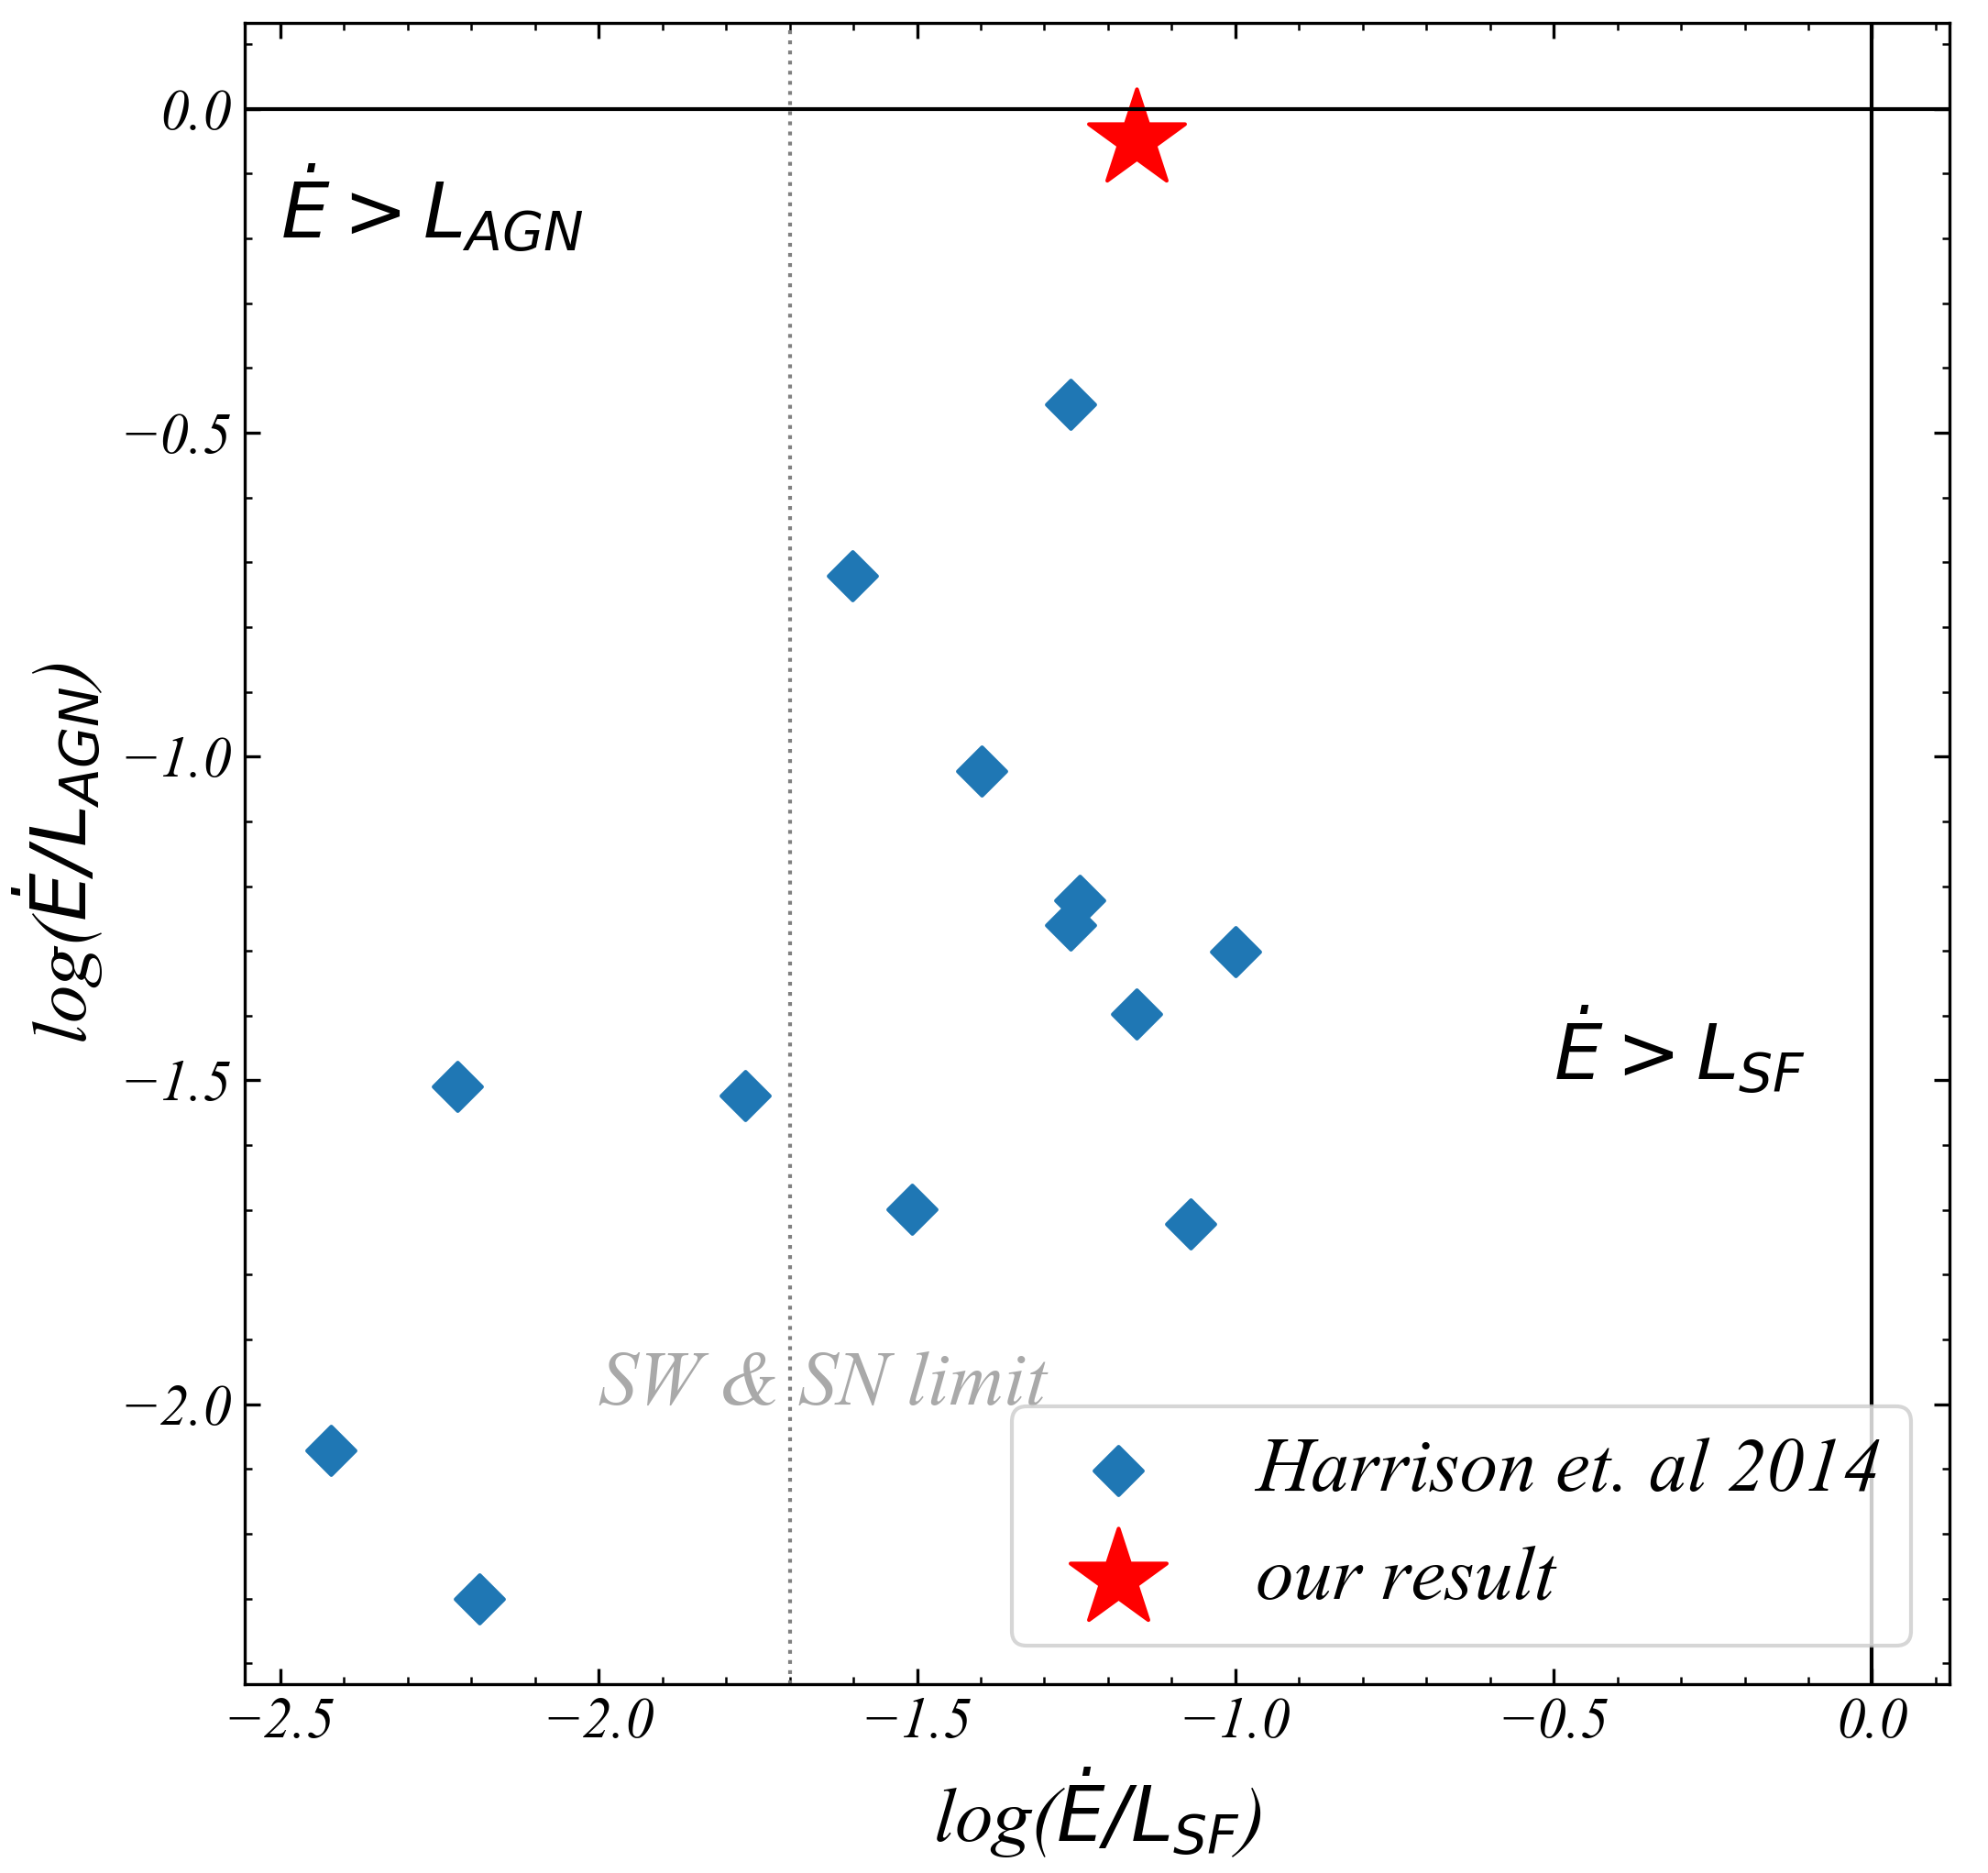
\includegraphics[width=0.5\textwidth]{figs/cp_AGN_vs_cp_SF}}
		\subfloat{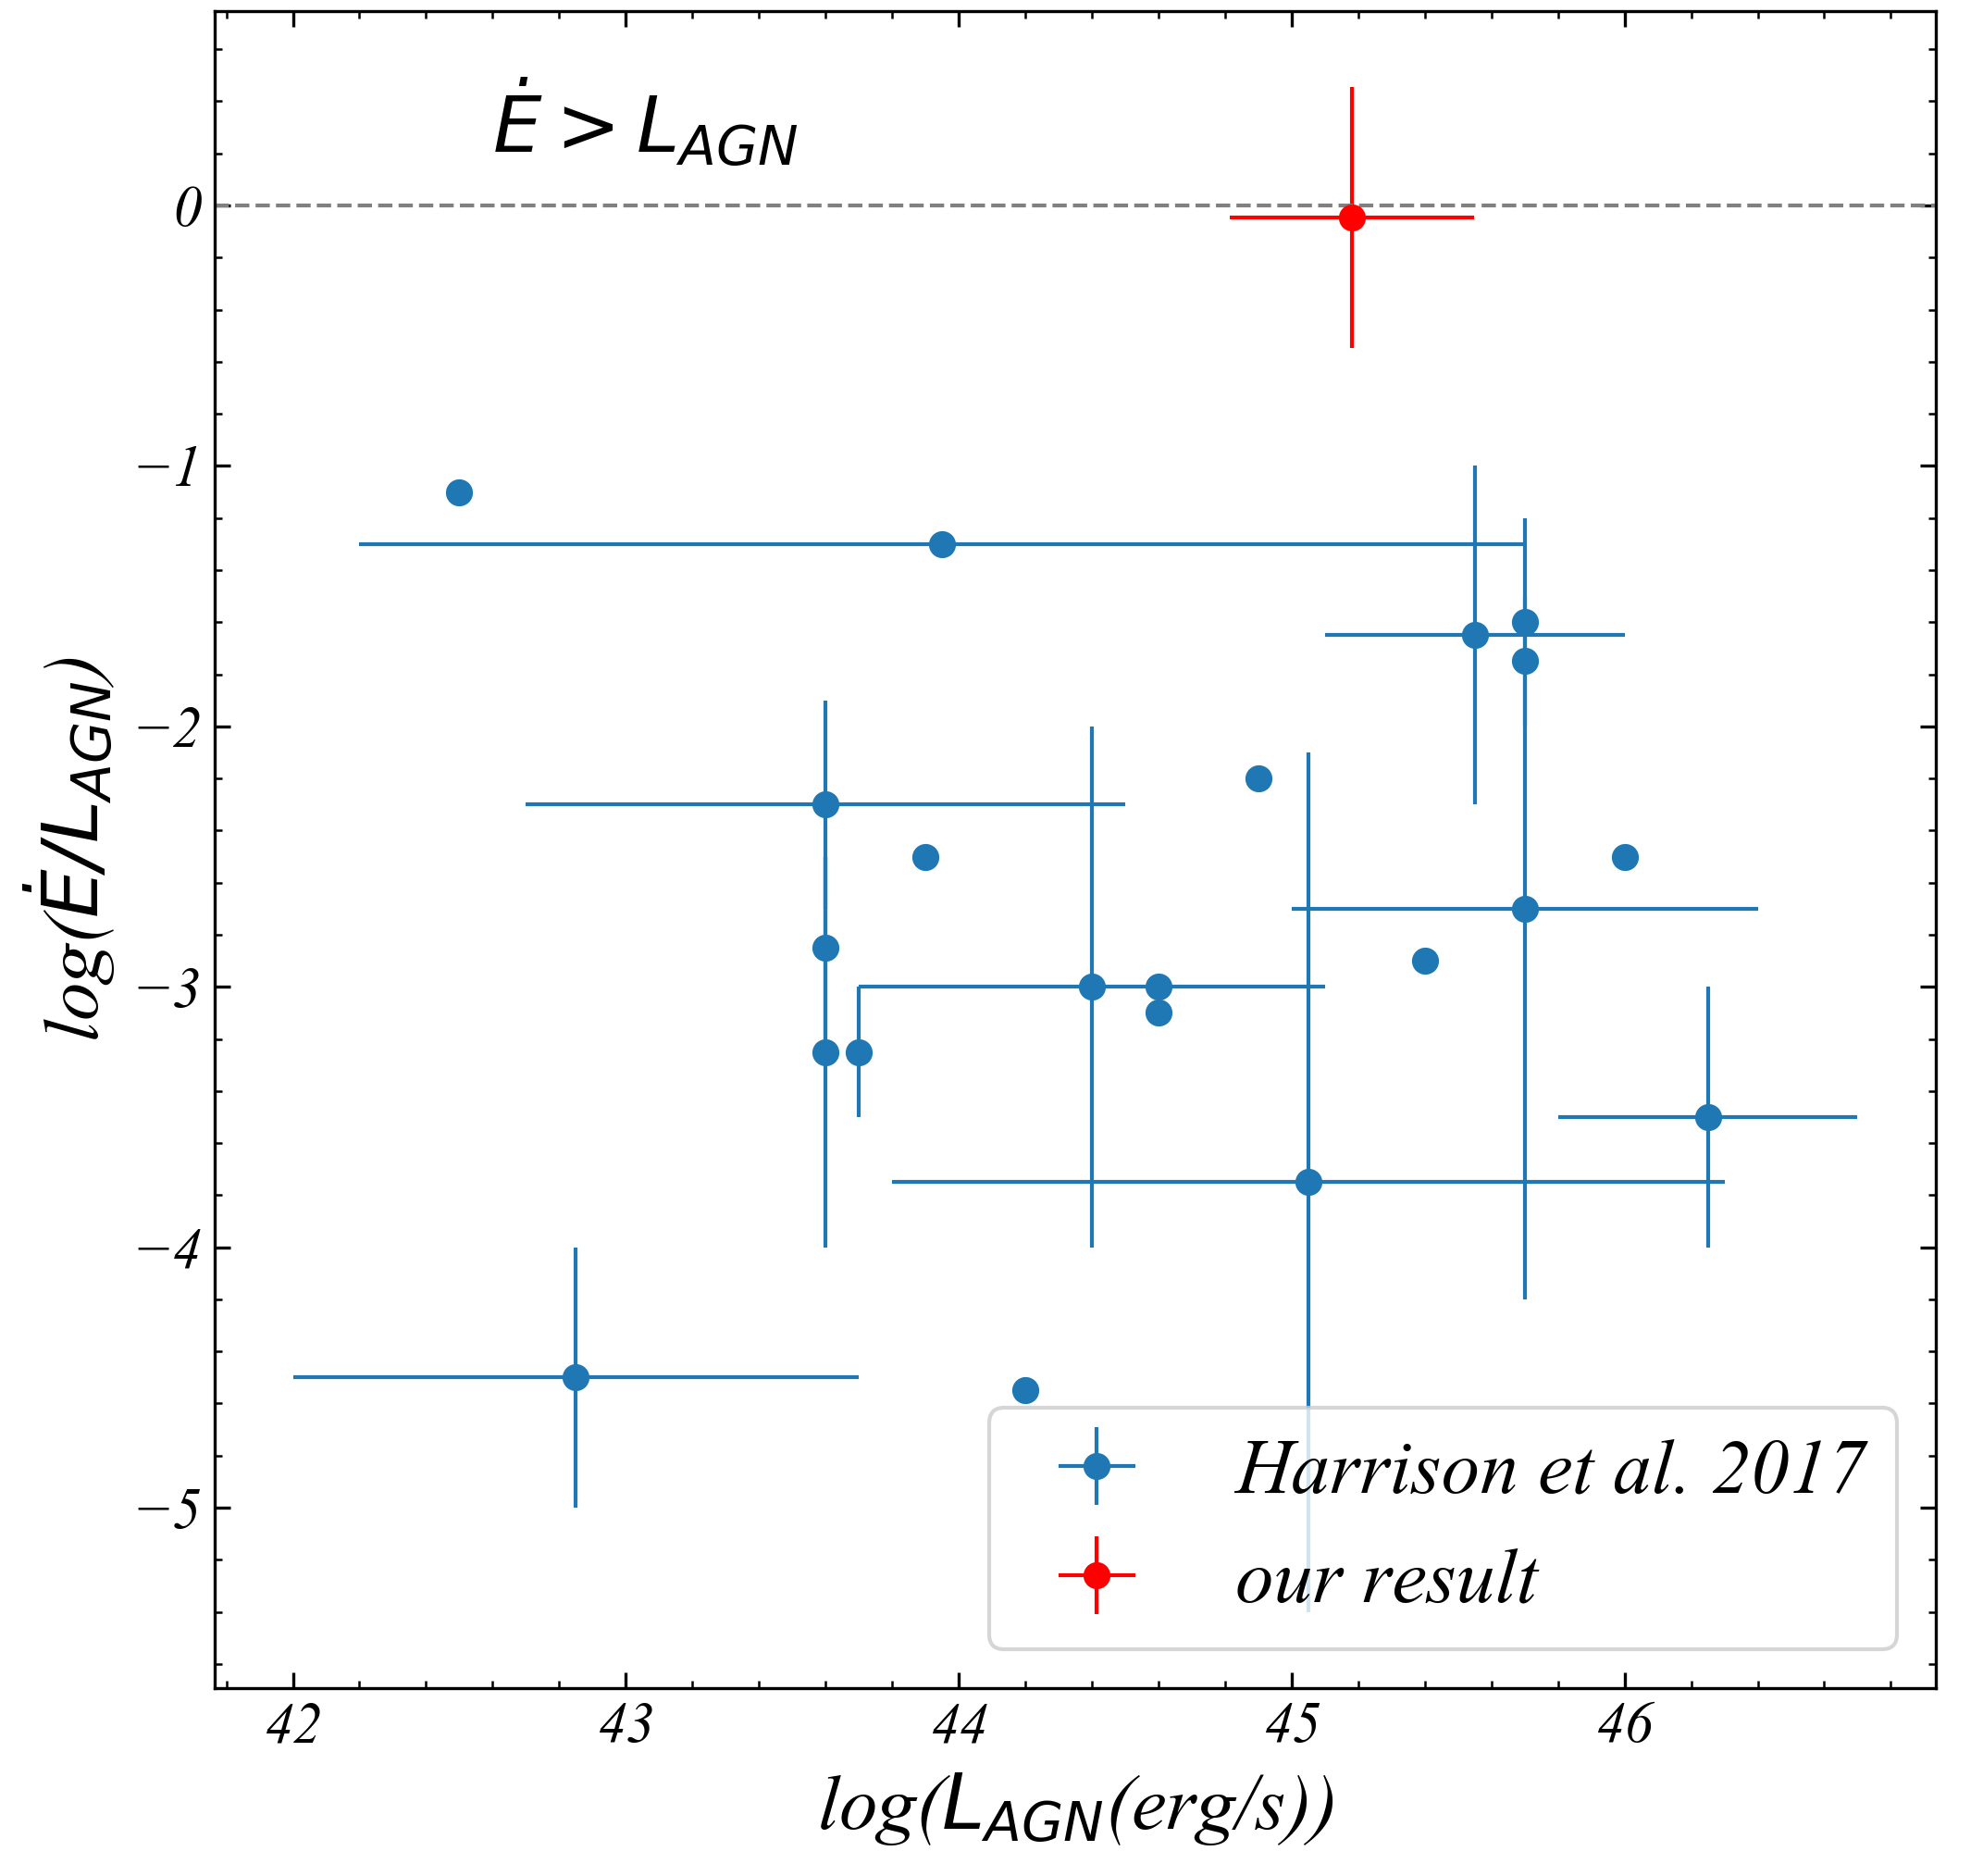
\includegraphics[width=0.5\textwidth]{figs/cp_AGN_vs_L_AGN}}
		\label{coupeffic}
		\caption{Left: the ratio of our estimated outflow kinetic energy rates($E_{out}$) to the AGN luminosity and to the star formation luminosity for our source(red) and sources from \cite{harrison2014kiloparsec}. The dashed vertical line is the estimated maximum mechanical input expected from supernovae and stellar winds. The two solid lines shows the coupling efficiency of 1. Right: Observationally determined kinetic coupling efficiencies in \cite{harrison2018agn} and our result. The vertical lines show the range of values quoted or, in the case of an error bar, the quoted error on the average value. The horizontal lines show the range of bolometric luminosity for each sample. The dotted line shows coupling efficiency of 1. }
	\end{figure*}
	
	In this section we will investigate which of these processes could responsible for driving the extreme outflows observed. The dominant processes that drive such large scale outflow in protocluster and the efficiency to which they are able to couple the gas are currently sources of uncertainty in galaxy formation models. Several possible mechanisms have been suggested to drive galaxy-wide outflows, for example: the stellar wind and supernovae; radiation pressure from the extremely luminous AGN or star formation; the interaction of radio jets with a clumpy and multiphase interstellar medium; AGN wind initially launched from the accretion disc. Following \cite{harrison2014kiloparsec}, we calculate the coupling efficiency which is a popular method to investigate the likely drivers of large-scale outflow. We compare the ratio of our outflow kinetic energy rate($\dot{E_{out}}$) with (1) the FIR AGN luminosity; (2) the FIR star formation luminosity (these two power are given by \cite{arrigoni2018qso}). We also calculate the momentum-loading factor for both star-forming-driven case and AGN-driven case. Using these results we now explore the possible driving mechanisms to power this outflow. 
	 
	 Fig.\ref{coupeffic} shows coupling efficiency for both star-forming-driven case and AGN-driven case. We compare our result with results in \cite{harrison2014kiloparsec}. One way for star formation to drive large-scale outflow is by stellar winds or supernovae. An estimation of the coupling efficiency for this case is carried by \cite{kennicutt1998star}, he found that the maximum coupling efficiency is $\dot{E_{out}}/L_{IR,SF} \approx 0.02$, we indicate this upper limit with gray dot line in Fig.\ref{coupeffic}. Based on this results, stellar winds and supernovae are unlikely to be fully responsible for the observed outflows. On the other hand, the coupling efficiency for AGN-driven case is too large which is close to 1. In the right panel of Fig.\ref{coupeffic} it shows that if the outflow is driven by AGN, it has already exceed other results with similar AGN luminosity. 
	 
	 Besides, if we instead consider a momentum-driven wind with momentum deposition from the radiation pressure of stars or AGN, the momentum loading factor $f_{p}=log(c\dot{P_{out}}/L)$ is $f_{p,SF}=1.7$ and $f_{p,AGN}=3.2$ respectively. Nevertheless \cite{zubovas2018agn} suggests that a typical momentum loading factor for star-formation-driven case is $f_{p,SF}< 1.4$ which is lower than our estimation, this comparison also rules out the star-formation case. In the same way, we also find that $f_{p,AGN}$ is larger than the typical value. 
	 
	 Moreover, \cite{shankar2006new} mentions the two sources of feedback are important over different mass ranges, in particular, stellar feedback regulates the processes in low-mass galaxies while large galaxies are mainly regulated by AGN feedback. The transition mass for this two feedback mechanisms is $M_{tr} \approx 2 \times 10^{10} \mathrm{M}_{\odot} $. By fitting the SED of source-B, \cite{arrigoni2018qso} estimates its stellar mass of source-B to be $\log \left(M_{\mathrm{star}} / \mathbf{M}_{\odot}\right)=11.4_{-0.2}^{+0.3}$. Comparing with $M_{tr}$, this results also suggests that feedback from star formation is not the dominant reason for the outflow.  
	 
	 However, \cite{zubovas2018agn} also suggests there are mechanisms to reach high coupling efficiency and momentum loading factor. One possibility is hyper-Eddington SMBH growth during Compton-thick(heavily obscured) phases. In this case, SMBH would accrete material with extremely large rate and may lead to ultra fast outflows(UFO).  \cite{tombesi2013unification} shows that this outflow can reach the velocity $\approx 0.1c$ and will have a strong coupling with the interstellar medium(ISM). Fig.6 of  \cite{tombesi2013unification} shows some coupling efficiency of some UFOs $\approx 1$, but he also explains that this extremely fast and powerful outflow would occur only very close to SMBH $R \approx 1000r_{s}$(where $r_{s}$ is the schwarzschild radius.).  He indicates that the large coupling efficiency is probably due to large environment column density $\approx 10_{24} cm^{-2}$ and highly ionized state. These two factors are consistent with the large-scale environmental conditions(MAMMOTH-1, extreme onverdensities; enomous lyman$\alpha$ nebula.). Nevertheless, \cite{cai2017discovery} suggests that the hydrogen column density is in the range $\approx 10^{20} cm^{-2}$, we indicate here that the column density in CGM maybe $10^{3} cm^{-2}$ larger than this value. 
	 
	 In summary, based on our analyses we find the outflow is unlikely powered by star-forming processes, but we do see some similar behaviors between the outflow and UFO(high coupling efficiency and high momentum loading factor), so we conclude that this outflow maybe driven by accretion-disc winds. Although there's large uncertainty coupling efficiency estimation, this large coupling efficiency and momentum loading factor have never been seen on such a large scale. From the observation it's still unclear what kind of mechanism leads to such large coupling efficiency on such large scale(the typical coupling efficiency beyond 10kpc <0.01), it maybe results from large column density $>10^{24}cm^{-2}$ or very efficient cooling mechanism. Besides, it provides evidence that outflow from central quasar can truely have influence on the protocluster.

\subsection{Galaxies merger}

By the submillimeter observation with ALMA and data collection from literature, \cite{arrigoni2018qso} fits the spectral energy distribution(SED) for Source-B, as a results he indicates that Source-B is an Ultra-Luminous Infrared Galaxy(ULIRG) with extreme far-infared luminosity. Besides, \cite{treister2010major} shows that there is substantial observational evidence that ULIRGs(heavily obscured galaxies) are the product of the gas-rich merger of two massive galaxies. \cite{cai2017discovery} also shows Source-B is a strongly obscured source. On the other hand the the flux-weighted dispersion map of ly$\alpha$ emission also shows velocity dispersion $ >600 km/s$ corresponding to FWHM $>1400 km/s$ near Source-B and the large dispersion extent to projected scale $\approx 100 kpc$(include G-5). Moreover, MAMMOTH-1 is an extreme overdensity($\delta =10.8 \pm 2.6$), The three sources of source-B is within 70 kpc. All of these evidences suggests a strong galaxies merger in this region. 
	
	We suggest that the physical picture of this area is like this: three sources of source-B is experiencing galaxy merger, center source accretes gas and material the other two sources, its super massive black hole(SMBH) is going through a period of rapid growth and produce strong outflow. Owing to the tidal effect between the three sources, lots of material is pulled out from galaxies to CGM. This can also explain why there's such large coupling efficiency between outflow and environment. 
	
	Futhermore, from the velocity and dispersion map we see that the region with large dispersion extent to G-5 and there's also obvious velocity gradient on either side of G-5. This clue indicates that there may be also outflow from G-5. The large dispersion also support this point.  
	\begin{figure*}
		\centering
		\subfloat{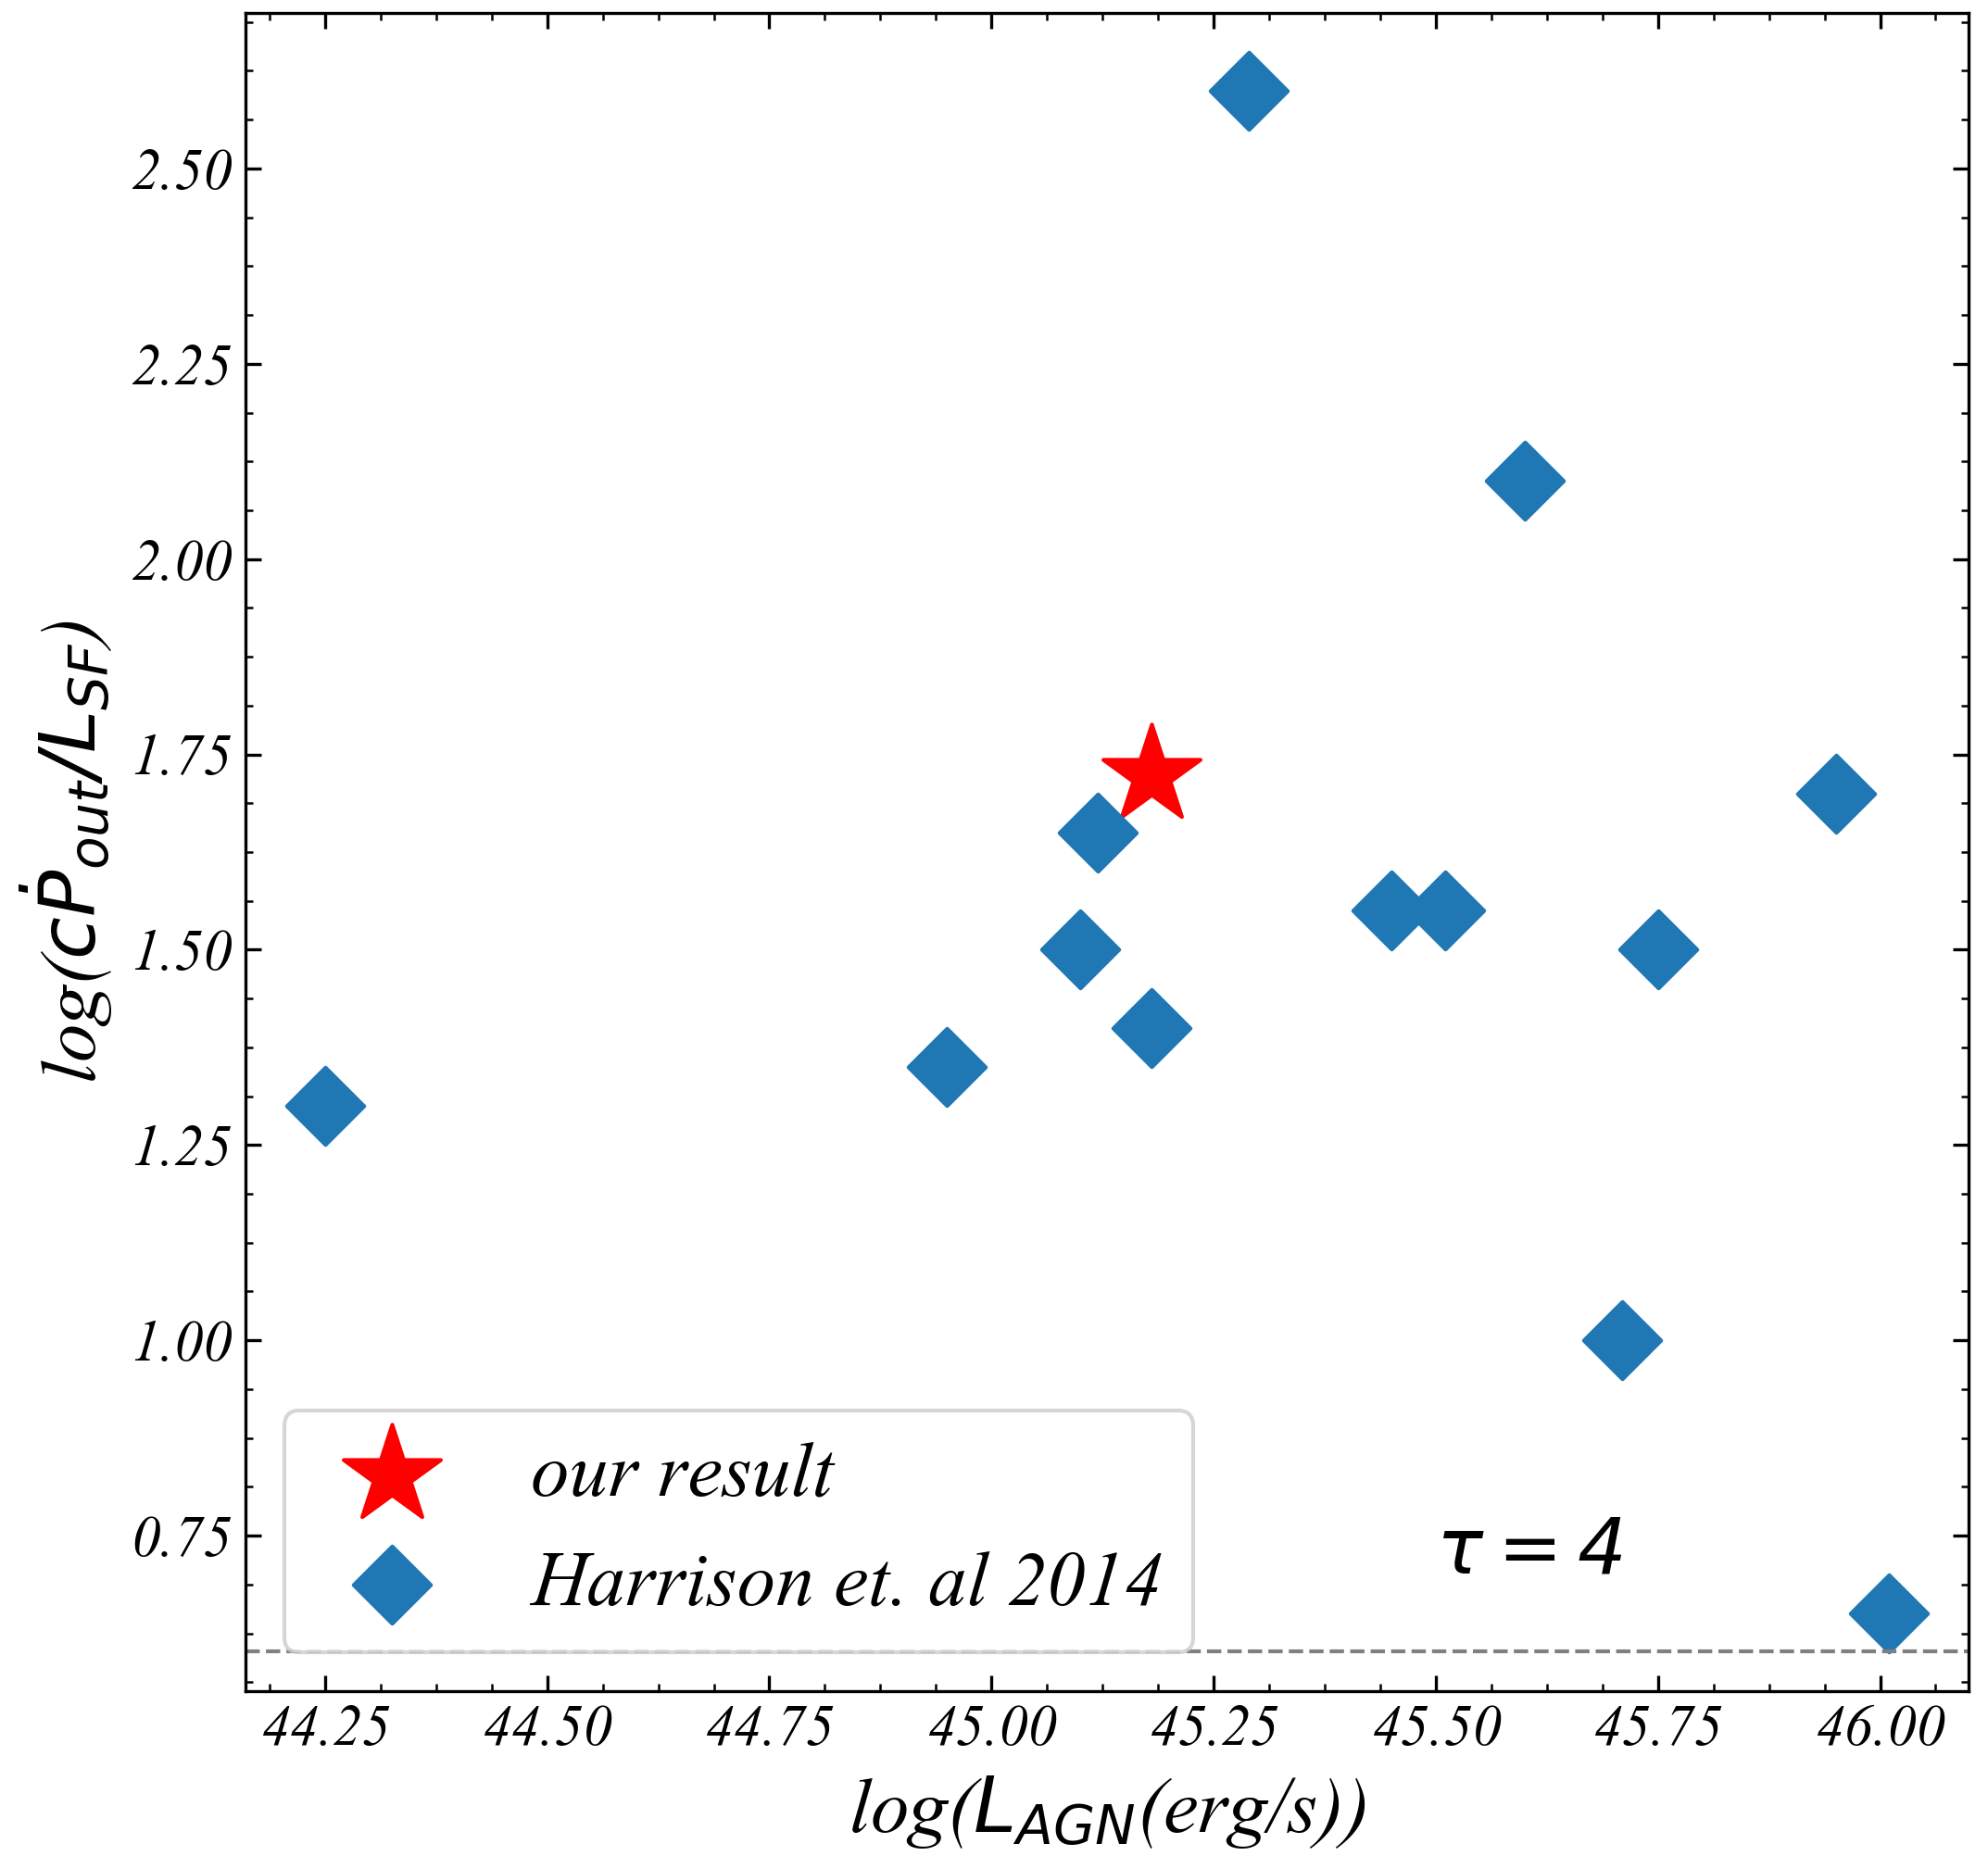
\includegraphics[width=0.5\textwidth]{figs/P_outSF_vs_L_AGN}}
		\subfloat{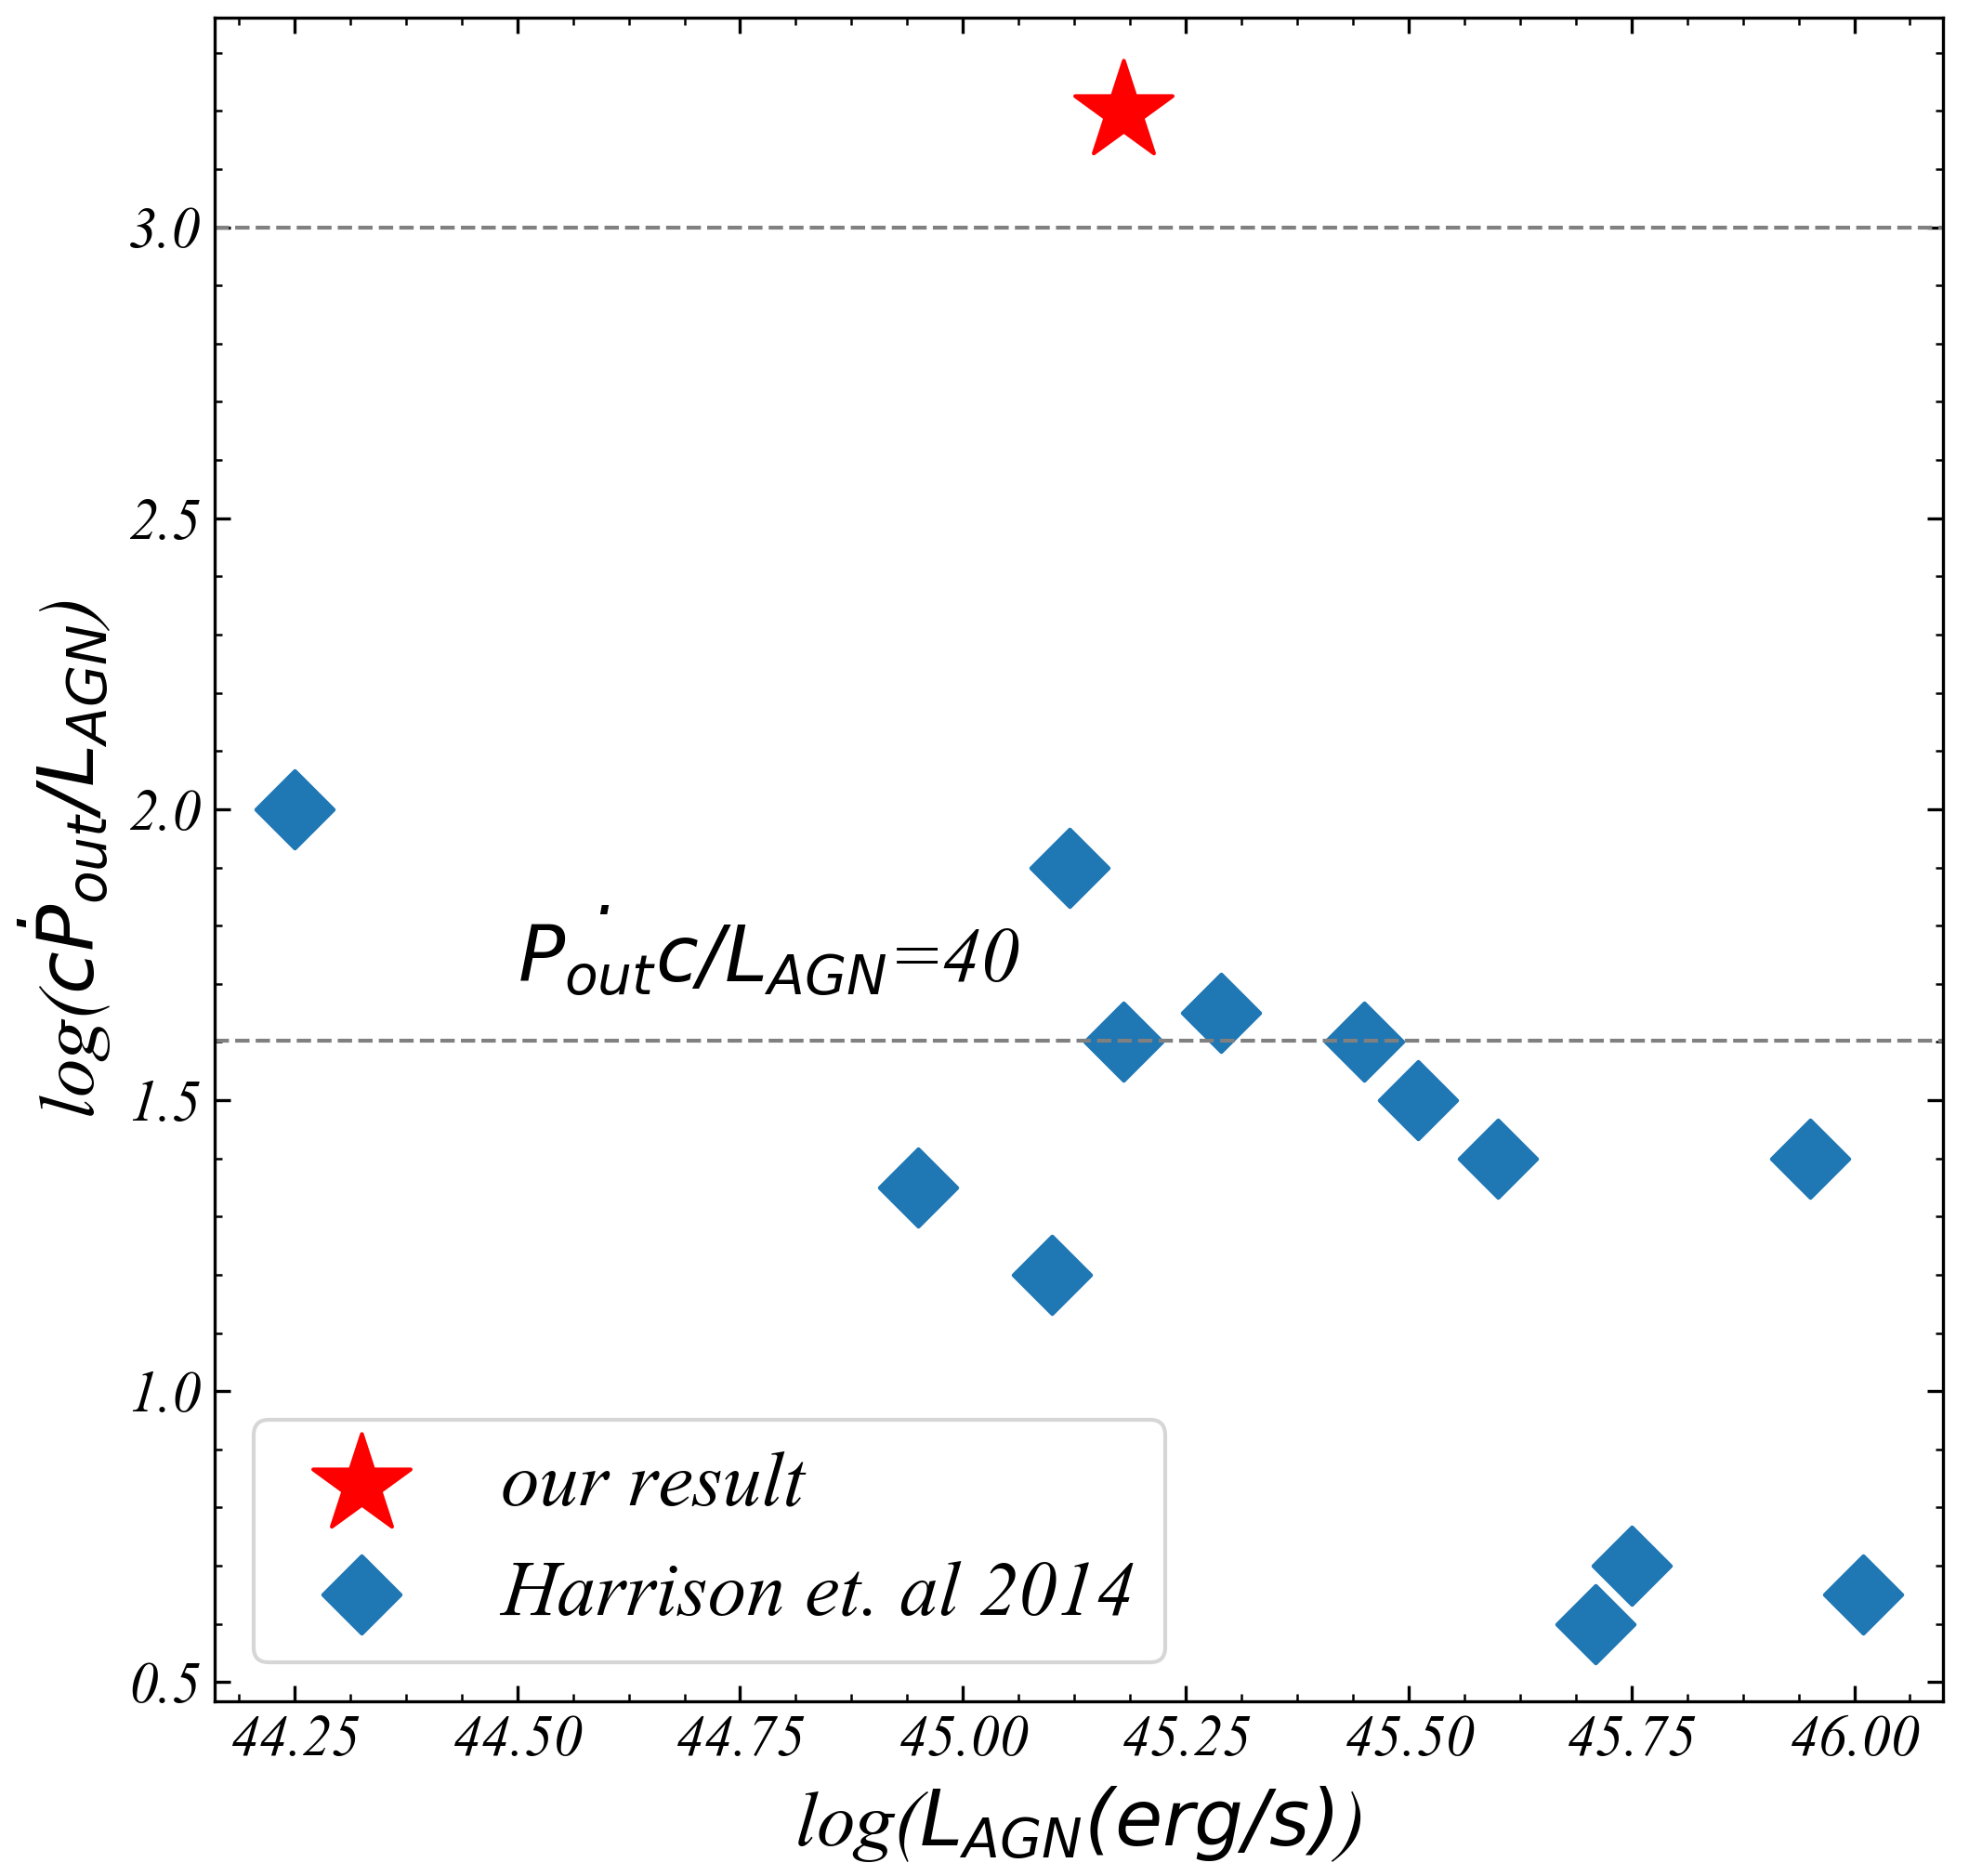
\includegraphics[width=0.5\textwidth]{figs/P_outAGN_vs_L_AGN}}
		\label{coupeffic}
		\caption{Left: momentum rates of the outflows($\dot{P_{out}}$ normalized to the star formation luminosity $L_{SF}/c$ versus AGN luminosity. The dashed lines represent the required optical depths if the outflows are driven by radiation pressure from star formation. Right: momentum rate of outflows normalized to AGN luminosity($L_{AGN}/c$) versus AGN luminosity. Based on our assumptions, the outflows are unlikely to be purely radiatively driven, the ratio is also to high for theoretical predictions of energy-driven outflows launched by AGN accretion-disc wind.}
	\end{figure*}

\section{Conclusions}
\label{sec:conclusions}

\acknowledgments


\bibliography{template}



\end{document}



%This section gives a scientific interpretation of the analyzed data.
%The \texttt{'\textbackslash micro'} macross provides the unslanted mu,
%`{\micro}' to be used for units of values, for example: {\micron} or
%{\microbar}.  Another nice feature are \texttt{'\$\textbackslash
%  ttt\{n\}\$'} for a 'ten-to-the-n' ($\ttt{n}$) and
%\texttt{'\$\textbackslash tttt\{n\}\$'} for 'times-ten-to-the-n'
%($\tttt{n}$).
%
%Table \ref{table:parameters} is a table.  Tables are well behaved;
%most of the time they appear right (or close to) where you put them.
%Figures are not.  The can show up anywhere in the pdf.   Be patient.
%
%\begin{table}[ht]
%\centering
%\caption{\label{table:parameters} Light curve parameters}
%\begin{tabular}{lc}
%\hline
%\hline
%Parameter                           & Value           \\
%\hline
%Eclipse depth (counts)              & 98.1            \\
%Eclipse duration (phase)            & 0.1119          \\
%Eclipse mid point (phase)           & 0.5015          \\
%Eclipse ingress/egress time (phase) & 0.013           \\
%Ramp slope (counts/phase)           & 0.006           \\
%System flux (counts)                & 25815           \\
%\hline
%% SOURCE: /home/patricio/ast/esp01/analyses/ligtcurve/attempt_547/results.txt
%\end{tabular}
%\end{table}
%
%
%Deluxe tables, like Table \ref{table:allplanets} are great. If they
%are too long, they automatically split and continue in the next
%page. Everything looks fine in Aastex6; however, in emulateapj the
%format seems to fail.
%Deluxe table may be a bit tricky. If you surround it with the table
%environment, you can specify where to place them (e.g., top, bottom).
%However, if you do, long tables wont automatically break into separate
%pages.  So, there is a trade off.
%
%%\begin{table}[t]
%% deluxetable works well for aastex6, not so much for emulateapj:
%\begin{deluxetable*}{lr@{}lr@{}lrrccrrrccrr}
%\tabletypesize{\footnotesize}
%%\tablecolumns{14}
%%\tablewidth{\textwidth}
%\tablecaption{Planets \label{table:allplanets}}
%
%\tablehead{\colhead{Name}                          &
%           \multicolumn{2}{c}{Mass}                &
%           \multicolumn{2}{c}{Radius}              &
%           \colhead{\Teq}                          &
%           \colhead{$\Omega$}                      &
%           \colhead{$a$}                           &
%           \colhead{$M$\sb{s}}                     &
%           \colhead{Age}                           &
%           \colhead{$\Omega\sb{\rm rot}$}          &
%           \colhead{Flux}                          &
%           \colhead{$L\sb{\rm h}$}                 &
%           \colhead{$L\sb{\rm e}$}                 &
%           \colhead{$L\sb{\rm h}$/$L\sb{\rm e}$}   &
%           \colhead{Ref.\,\tnm{a}}                 \\
%           \colhead{}                              &
%           \multicolumn{2}{c}{\mearth}             &
%           \multicolumn{2}{c}{\rearth}             &
%           \colhead{}                              &
%           \colhead{}                              &
%           \colhead{}                              &
%           \colhead{\msun}                         &
%           \colhead{}                              &
%           \colhead{$\Omega\sb{\odot}$}            &
%           \colhead{erg\,s$\sp{-1}$\,cm$\sp{-2}$}  &
%           \colhead{s$\sp{-1}$}                    &
%           \colhead{s$\sp{-1}$}                    &
%            \colhead{}                              }
%\startdata
%55 Cnc e      & $ 8.38$ & $\pm 0.39$               & $ 2.08$ & $\pm 0.16$             &         1957 &       15.6 & $0.015$ & $0.91$ & $  10.2$ & $1.4$ & $142697.6$ & $3\times10^{30}$ & $3\times10^{30}$ & $\cdots$ & De11 \\
%55 Cnc e      & $ 8.38$ & $\pm 0.39$               & $ 2.08$ & $\pm 0.16$             &         1957 &       15.6 & $0.015$ & $0.91$ & $  10.2$ & $1.4$ & $142697.6$ & $\cdots$ & $\cdots$ & $\cdots$ & De11 \\
%55 Cnc e      & $ 8.38$ & $\pm 0.39$               & $ 2.08$ & $\pm 0.16$             &         1957 &       15.6 & $0.015$ & $0.91$ & $  10.2$ & $1.4$ & $142697.6$ & $\cdots$ & $\cdots$ & $\cdots$ & De11 \\
%55 Cnc e      & $ 8.38$ & $\pm 0.39$               & $ 2.08$ & $\pm 0.16$             &         1957 &       15.6 & $0.015$ & $0.91$ & $  10.2$ & $1.4$ & $142697.6$ & $\cdots$ & $\cdots$ & $\cdots$ & De11 \\
%\enddata
%% The minipage environment keeps the table footer within the page
%% width when the table occupies the full width.
%% Use \vspace to adjust latex quirks with the vertical spacing.
%%\begin{minipage}{\textwidth}%\vspace{0.4cm}
%\tablenotetext{a}{
%Lorem Ipsum is simply dummy text of the printing and typesetting industry. Lorem Ipsum has been the industry's standard dummy text ever since the 1500s, when an unknown printer took a galley of type and scrambled it to make a type specimen book. It has survived not only five centuries, but also the leap into electronic typesetting, remaining essentially unchanged. It was popularised in the 1960s with the release of Letraset sheets containing Lorem Ipsum passages, and more recently with desktop publishing software like Aldus PageMaker including versions of Lorem Ipsum.
%}
%%\end{minipage}
%\end{deluxetable*}
%%\end{table}
